% \documentclass{article}


% \usepackage[natbibapa,nodoi]{apacite}
% %\usepackage{natbib}
% \usepackage{arxiv}
% \usepackage[utf8]{inputenc} % allow utf-8 input
% \usepackage[T1]{fontenc}    % use 8-bit T1 fonts
% \usepackage[colorlinks=true, citecolor = blue]{hyperref}      % hyperlinks
% \usepackage{url}            % simple URL typesetting
% \usepackage{booktabs}       % professional-quality tables
% \usepackage{amsfonts}       % blackboard math symbols
% \usepackage{nicefrac}       % compact symbols for 1/2, etc.
% \usepackage{microtype}      % microtypography
% \usepackage{graphicx, subfigure}
% \usepackage{lipsum}
% \usepackage{amsmath}
% \usepackage{amsthm}
% \usepackage{amssymb}
% \usepackage{import}
% \usepackage{enumitem}
% \usepackage{csquotes}
% \usepackage{todonotes}
% \usepackage{xfrac}
% \usepackage{wasysym}

% %%% ============================================================================
% %%% Theorems.
% %%% ============================================================================
% \theoremstyle{plain}
% \newtheorem{thm}{\protect\theoremname}
% \theoremstyle{plain}
% \newtheorem{lem}{\protect\lemmaname}
% \theoremstyle{definition}
% \newtheorem{defn}[thm]{\protect\definitionname}
% \theoremstyle{remark}
% \newtheorem{rem}[thm]{\protect\remarkname}
% \theoremstyle{definition}
% \newtheorem{example}[thm]{\protect\examplename}
% \theoremstyle{plain}
% \newtheorem{cor}[thm]{\protect\corollaryname}
% \theoremstyle{plain}
% \newtheorem{prop}[thm]{\protect\propositionname}
% \theoremstyle{definition}
% \newtheorem{xca}[thm]{\protect\exercisename}
% \ifx\proof\undefined
% \newenvironment{proof}[1][\protect\proofname]{\par
% 	\normalfont\topsep6\p@\@plus6\p@\relax
% 	\trivlist
% 	\itemindent\parindent
% 	\item[\hskip\labelsep\scshape #1]\ignorespaces
% }{%
% 	\endtrivlist\@endpefalse
% }
% \providecommand{\proofname}{Proof}
% \fi

% \providecommand{\corollaryname}{Corollary}
% \providecommand{\definitionname}{Definition}
% \providecommand{\propositionname}{Proposition}
% \providecommand{\examplename}{Example}
% \providecommand{\exercisename}{Exercise}
% \providecommand{\remarkname}{Remark}
% \providecommand{\theoremname}{Theorem}
% \providecommand{\lemmaname}{Lemma}

\documentclass[twoside]{article}
\usepackage{moss} % contains layout and most imported packages.


%%% ============================================================================
%%% Macros.
%%% ============================================================================
\DeclareMathOperator{\tr}{tr}
\DeclareMathOperator{\Tr}{Tr}
\DeclareMathOperator{\Var}{Var}
\DeclareMathOperator{\sd}{sd}
\DeclareMathOperator{\argmin}{argmin}
\DeclareMathOperator{\Cor}{Cor}
\DeclareMathOperator{\Cov}{Cov}
\DeclareMathOperator{\diag}{diag} 
\DeclareMathOperator{\MSE}{MSE} 
\DeclareMathOperator{\tsum}{\textstyle \sum}

\renewcommand{\sqrt}[1]{{(#1)^{1/2}}}

\DeclareMathOperator{\argmax}{argmax}

\title{Please avoid the standardized alpha}

\author{
  Jonas Moss \orcid{0000-0002-6876-6964} \\
  Department of Mathematics, University of Oslo\\
  PB 1053, Blindern, NO-0316, Oslo, Norway \\
  \it{jonasmgj@math.uio.no}
}

\titletag{An PsyArXiv preprint, v1.0}
\makeatletter
\titlerunning{\@title}
\makeatother
\authorrunning{Jonas Moss}

\begin{document}
\maketitle

\begin{abstract}
Coefficient alpha is the most widely used measure of reliability for psychometric instruments. A cousin of coefficient alpha is the standardized alpha, which is calculated from the correlation matrix instead of the covariance matrix. I argue coefficient alpha should always be preferred over the standardized alpha. For coefficient alpha is often consistent when the standardized alpha fails to be, but the opposite is rarely the case. Moreover, assuming normality, coefficient alpha and standardized alpha have the same asymptotic efficiency under the parallel model, the only case when both are consistent. Since coefficient alpha is the maximum likelihood estimator under the normal parallel model, the only reason to prefer the standardized coefficient would be if it had superior small-sample performance. But a small simulation study shows the two alphas perform equally well under small samples. I argue against the ordinal alpha, a cousin of standardized alpha based on the polychoric correlation matrix, and propose an alternative.
\end{abstract}

% keywords can be removed
\keywords{reliability \and coefficient alpha \and Cronbach's alpha}

\section{Introduction}

((Smoother introduction.))

In unidimensional psychometric scales with $k$ test items, the most popular predictor $\hat{Z}$ is the sum of test items, $\hat{Z}=X_1 + \cdots + X_k$. This predictor is often called the sum score \citep{McNeish2019-ea}, and the associated reliability is the congeneric reliability \citep{Cho2016-bs}. The sample coefficient alpha is the most popular estimator of the congeneric reliability, and so it has been for a long time \citep{McNeish2018-vu}. A close cousin of coefficient alpha is the standardized coefficient alpha, or standardized alpha for short. The difference between these two alphas is simple: To calculate coefficient alpha you use the covariance matrix, to calculate the standardized alpha you use the correlation matrix.

I argue you should avoid standardized alpha in all circumstances. I make my case with two arguments:

\begin{enumerate}[label=(\Alph*)]
\item I compare standardized alpha to the coefficient alpha as estimators of the congeneric reliability. Standardized alpha is reasonable estimator of the congeneric only under the parallel model, but I argue you should prefer coefficient alpha even if you have good reasons to believe in the parallel model. While the population values of standardized alpha and coefficient alpha equals the congeneric reliability under the parallel model, coefficient alpha equals the congeneric reliability under the more general $\tau$-equivalent model. But standardized alpha will be greater than the congeneric reliability under the $\tau$-equivalent model. Moreover, sample coefficient alpha is the maximum likelihood estimator of the congeneric reliability under the parallel model with multivariate normal errors and normal latent variables, which provides a decent heuristic argument in favor of coefficient alpha. Finally, provided the observed variables have finite fourth moments, sample coefficient alpha and sample standardized alpha have the same asymptotic variances. 

\item A common stance on sample standardized alpha is to use it only with standardized test scores. In this case, sample standardized alpha is best understood as an estimator of the standardized reliability, i.e. the squared correlation between $Z$ and $\hat{Z}$ when $\hat{Z}$ is the sum of standardized test items. However, the standardized alpha equals the standardized reliability only under restrictive and unrealistic conditions. If you are willing to go for another kind reliability than the congeneric reliability, consider coefficient $H$ instead, which corresponds to the optimal linear predictor $\hat{Z}$. If coefficient $H$ is too hard to swallow, I propose to standardize with the the residual errors and use the new sigma reliability.
\end{enumerate}

In section \ref{sec:coefficienta alpha} I introduce coefficient alpha, the standardized alpha, and the notion of reliability. I make an effort to be mathematically precise here, and reiterate several known properties about the alphas in Proposition \ref{prop:Reliabilities.}. I elaborate on argument A in section \ref{sec:argument A} and devote section \ref{sec:argument B} to argument B. In section \ref{sec:Ordinal alpha} I argue against the use of the ordinal alpha of  \citet{Zumbo2007-ap} and propose an alternative.

% I end with some brief remarks in section \ref{sec:remarks}.
\section{Coefficient alpha and standardized alpha}
\label{sec:coefficienta alpha}

Let $X$ be random variable in $\mathbb{R}^{k}$ with finite variance.
Let $\Sigma=\Cov X$ be the covariance matrix of $X$ and $\Phi=\Cor X$
be the correlation matrix of $X$. Let $\mathbf{i}=(1,1,\ldots,1)$ by a vector of ones of the appropriate size and $\tr$ be the trace operator.
The population coefficient alpha \citep[][eq. 2]{cronbach1951coefficient} is
\begin{equation}
\alpha =  \frac{k}{k-1}\left(1-\frac{\tr\Sigma}{\mathbf{i}^{T}\Sigma\mathbf{i}}\right)\label{eq:Coefficient alpha}
\end{equation}
and the population standardized alpha \citep[][eq. 2]{Falk2011-ae} is
\begin{equation}
\alpha_S=\frac{k}{k-1}\left(1-\frac{k}{\mathbf{i}^{T}\Phi\mathbf{i}}\right)\label{eq:standardized alpha}
\end{equation}
We care about these alphas since they sometimes coincide with the reliability coefficient under the congeneric model, a special case of the linear one-factor model. Let $Z$ be a mean zero latent variable with unit variance and $\varepsilon=(\varepsilon_{1},\varepsilon_{2},\ldots,\varepsilon_{k})$
be a mean zero vector of uncorrelated errors with unit variance. In addition, assume $Z$ and $\varepsilon$ are uncorrelated. Define the congeneric model
\begin{equation}
X=\lambda Z+\Psi^{1/2}\varepsilon\label{eq:congeneric model}
\end{equation}
where $\lambda$ is a vector of loadings, and $\Psi^{1/2}$ is a diagonal matrix with positive diagonal elements $\sigma_i$. Since $\Psi^{1/2}$ is diagonal the errors $\Psi^{1/2}\varepsilon$ are uncorrelated. When $\Psi^{1/2}$ is allowed to be any positive definite matrix, the model \eqref{eq:congeneric model} is a one-factor model, and if the dimension of $Z$ is larger than one it is a linear factor model. The random variables $Z$ and $\varepsilon$ can have any distribution whatsoever. Since $\lambda,\Psi$ are parameters of the model, we are dealing with a semi-parametric model. 

The congeneric model is not necessarily a realistic model. The assumption of one latent factor $Z$ and the assumption of uncorrelated errors are unrealistic in most psychometric settings \citep[][section 1.2 -- 1.3]{Green2009-le}. I have restricted this paper to the congeneric model since it is commonly used, standardized alpha only makes sense on specific cases of the congeneric models, and it makes the presentation smoother. Nevertheless, if I were to use a general linear factor model, the case against standardized alpha as a reliability coefficient would be even stronger. See \citet[][section 2]{Green2009-le} for an assessment of how coefficient alpha fares when the congeneric model assumption is loosened up.

It is time to define reliability. Let $Z$ be an unobserved variable and $\hat{Z}$ a prediction of $Z$. The reliability coefficient is the squared correlation between a latent variable $Z$ and its predictor $\hat{Z}$ \citep[][p. 61]{Lord1968-ax}. 

\begin{defn}\label{defn:reliability} The reliability of $\hat{Z}$ as a predictor of $Z$ is $\omega=\Cor^{2}(\hat{Z},Z)$.
\end{defn} 

The squared correlation between two variables $X$ and $Y$ quantifies the degree of linear relationship between $X$ and $Y$, with $0$ being no linear relationship and $1$ a perfect linear relationship. In the same way, the reliability coefficient quantifies how well the noisy $\hat{Z}$ works as a predictor of $Z$.

In this paper the predictors $\hat{Z}$ are linear functions of $X$, that is, there are some real weights $w_{i},i=1,\ldots,k$, such that
\begin{equation}
\label{eq:Linear predictor}
\hat{Z} =  \sum_{i=1}^{k} w_{i}X_i = \sum_{i=1}^{k}w_{i}(Z\lambda_i + \sigma_{i} \varepsilon_i).\nonumber 
\end{equation}
The second equation follows from the definition of $X$ in the congeneric model \eqref{eq:congeneric model}. 

%Since $\hat{Z}$ is determined by its weights $w_i$, I will sometimes talk about the reliability with weights $w_i$.

The purpose of the reliability coefficient is to tell us how well a linear predictor $\hat{Z}$ predicts $Z$. In this sense it is analogous to $R^2$ from linear regression. The following proposition makes this claim precise. In this proposition, and the rest of the paper, I will use the notation $\overline{x}$ to denote the mean of the vector $x$. Moreover, when $x$ and $y$ are vectors of the same length, $xy$ is the pointwise product of $x$ and $y$.

\begin{prop}
\label{prop:reliability motivation}Assume the congeneric model \eqref{eq:congeneric model}. Let $\hat{Z}=\sum_{i=1}^{k}w_{i}X$
for some vector of weights $w$ with elements $w_{i},i=1,\ldots,k$. Then the reliability equals
\begin{eqnarray}
\omega & = & \frac{(w^{T}\lambda)^{2}}{(w^{T}\lambda)^{2}+w^{T}\Psi w}\label{eq:linear reliabiltiy}\\
 & = & \frac{(w^{T}\Sigma v)^{2}}{w^{T}\Sigma w} \nonumber \\
 & = & 1- \MSE (w_{0}\hat{Z})\nonumber 
\end{eqnarray}
where $\MSE (w_{0}\hat{Z})=E[(Z-w_{0}\hat{Z})^{2}]$ is the
mean squared error, $w_{0}=\overline{w\lambda}/(k\overline{w\lambda}^{2}+\overline{w^{2}\sigma^{2}})$ is the constant minimizing the mean squared error, and  $v_{i}=\lambda_{i}/[\sigma_{i}^{2}(1+k\overline{\lambda^{2}\sigma^{-2}})],\:i=1,\ldots,k$ are the Thurstone weights.
\end{prop}
\begin{proof}
See the appendix, page \pageref{proof:reliability motivation} for a proof.
\end{proof}

Equation \eqref{eq:linear reliabiltiy} is the definition \citet[][p. 112]{Joreskog1971-nn} gave of the composite reliability under the congeneric model \eqref{eq:congeneric model}. The role of $w_0$ in Proposition \ref{prop:reliability motivation} is to make sure $\hat{Z}$ predicts $Z$ on he right scale, and in this paper the scale of $Z$ is fixed by $\Var Z = 1$. Since $Z$ is latent we would usually not care about this scale, but it is handy to fix it to $1$ since it allows us to compare different predictors of $\hat{Z}$. The formulation $1-\MSE (w_{0}\hat{Z})$ is more concrete than the correlation formulation, as it explicitly references the predictor $w_{0}\hat{Z}$, while the correlation is scale-free and more abstract. The mean squared error definition is amenable to generalizations too, and I will explore one such generalization in a future paper. 

A modestly popular choice for $w$ are the weights minimizing the mean squared error, known as the Thurstone weights \citep{thurshronebook}. Using these weights lead to coefficient $H$ \citep{hancock2001rethinking}, also known as the maximal reliability \citep{Li1997-yh}, 
\begin{equation}
\label{eq:coefficient_H}
\omega_{H}=\frac{k\overline{\lambda^{2}\sigma^{-2}}}{k\overline{\lambda^{2}\sigma^{-2}}+1},
\end{equation}
where $\overline{\lambda^{2}\sigma^{-2}} = k^{-1}\sum_{i=1}^{k}\lambda_{i}^2/\sigma_i^2$. But by far the most popular choice is give to same weight to each $X_i$, that is, $w = \mathbf{i}=(1,1,\ldots,1)$. This leads to the congeneric reliability
\begin{equation}
\omega =\frac{k\overline{\lambda}^{2}/\overline{\sigma^{2}}}{k\overline{\lambda}^{2}/\overline{\sigma^{2}} + 1}\label{eq:Congeneric reliability}
\end{equation}
where $\overline{\lambda}=k^{-1}\sum_{i=1}^{k}\lambda_{i}$ and
$\overline{\sigma^{2}}=k^{-1}\sum_{i=1}^{k}\sigma_{i}^{2}$. Finally, the weights $w_i = \sqrt{\lambda_i^2 + \sigma_i^2}$ yield the standardized reliability, which is closely related to standardized alpha.
\begin{equation}
\omega_s=\frac{k\overline{\lambda(\lambda^{2}+\sigma^{2})^{-1/2}}^{2}/\overline{\sigma^{2}(\lambda^{2}+\sigma^{2})^{-1}}}{k\overline{\lambda(\lambda^{2}+\sigma^{2})^{-1/2}}^{2}/\overline{\sigma^{2}(\lambda^{2}+\sigma^{2})^{-1}}+1}.\label{eq:Standardized reliability}
\end{equation}
It is time to relate the reliabilities to the alpha coefficients.
Define the generalization of the coefficient alpha and the standardized
alpha, the \emph{weighted alpha},

\begin{defn}
Let $w$ be a vector of weights and $\Sigma$ a covariance matrix. The \textit{weighted alpha} is
\begin{equation}
\alpha_{w}=\frac{k}{k-1}\left(1-\frac{w^{T}(\diag\Sigma)w}{w^{T}\Sigma w}\right)\label{eq:weighted alpha}
\end{equation}
where $\diag\Sigma$ is the diagonal matrix with diagonal equal to the diagonal of $\Sigma$.
\end{defn}
The ordinary coefficient alpha \eqref{eq:Coefficient alpha} has weights $w=\mathbf{i}$
while the standardized alpha \eqref{eq:standardized alpha} has weights $w_{i}=\sqrt{\lambda_{i}^{2}+\sigma_{i}^{2}}$. Coefficient alpha and standardized alpha are the most interesting cases of the weighted alpha as you can calculate them using only the covariance matrix $\Sigma = \Cov X$, but the definition makes sense for any weight $w$. The following Proposition summarizes the basic relationship
between the reliability $\omega_{w}$ and the weighted $\alpha_{w}$. To state it, we will need
the notion of a \emph{$\tau$-equivalent model} \citep[][section 2.13]{Lord1968-ax}. A congeneric model \eqref{eq:congeneric model} is $\tau$-equivalent if $\lambda_{i}=\lambda_{j}$ for all $i,j$. That is, all unstandardized
factor loadings are equal.
\begin{prop}
\label{prop:weighted alpha}. Let $w$ be a vector of weights and
assume $X$ follows the congeneric model \eqref{eq:congeneric model}. Then 
\begin{equation}
\alpha_{w}=\omega_{w}-\frac{k}{k-1}\frac{\overline{w^{2}\lambda^{2}}-\overline{w\lambda}^{2}}{k\overline{w\lambda}^{2}+\overline{w^{2}\sigma^{2}}}\label{eq:alpha-omega discrepancy}
\end{equation}
and $\alpha_w \leq \omega_w$ with equality if and only if $wX$ is $\tau$-equivalent, i.e. $w_i\lambda_{i}=w_j\lambda_{j}$
for all $i,j$.
\end{prop}
\begin{proof}
This proposition is classical for the special case unit weights $w = \mathbf{i}$ \citep[][pp. 87 -- 89]{Lord1968-ax}. See the appendix page \pageref{proof:weighted alpha}
for a proof. The discrepancy term in \eqref{eq:alpha-omega discrepancy} for the special case of coefficient alpha is extensively discussed by \citet{Raykov1997-bu}. 
\end{proof}

% By Chebyshev's inequality, $k\overline{w\lambda}^{2}\geq\overline{(w\lambda)^{2}}$,
% with equality if and only if $w_{i}\lambda_{i}=w_{j}\lambda_{j}$,
% that is, the weighted model is $\tau$-equivalent. The discrepancy term in \eqref{eq:alpha-omega discrepancy} for the special case of coefficient alpha is extensively discussed by \citet{Raykov1997-bu}. 

Proposition \ref{prop:weighted alpha} is a minor generalization of the two most frequently mentioned fact about coefficient alpha: (i) That $\alpha = \omega$ under the $\tau$-equivalent model. (ii) Coefficient alpha is a lower bound for the congeneric reliability, $\alpha \leq \omega$ under the congeneric model.
 
When $w_{i}=\sqrt{\lambda_{i}^{2}+\sigma_{i}^{2}}$, $wX$ is $\tau$-equivalent if and only if the standardized factor loadings are equal, and Proposition \ref{prop:weighted alpha} tells us $\alpha_S = \omega_S$ in this case. 

The next proposition explores the relationship between coefficient alpha, the standardized alpha, and the congeneric reliability coefficient.

\begin{prop}
\label{prop:Reliabilities.}Assume the congeneric model \eqref{eq:congeneric model}. Let $\alpha$ be coefficient alpha \eqref{eq:Coefficient alpha}, $\alpha_S$ be the standardized alpha \eqref{eq:standardized alpha}, and  $\omega$ be the congeneric reliability \eqref{eq:Congeneric reliability}. 
\begin{enumerate}[label=(\roman*)]
\item Assume $\lambda_{i}=\lambda_{j}$ for all $i,j$, i.e. the $\tau$-equivalent model. Then $\alpha_S \geq \alpha = \omega$, with equality if and only if $\sigma_{i}=\sigma_{j}$ for all $i,j$ or $\lambda_i = 0$ for all $i$.
\item If $k=2$, $\alpha_S\geq\alpha$, with equality if and only if $\lambda_{1}^{2}+\sigma_{1}^{2}=\lambda_{2}^{2}+\sigma_{2}^{2}$ or $\lambda_1 = 0$ or $\lambda_2 = 0$. But if $k>2$, both $\alpha_S>\alpha$
and $\alpha_S<\alpha$ are possible.
\item All of $\alpha_S=\omega$, $\alpha_S>\omega$ and $\alpha_S<\omega$
are possible when $\lambda_{i}\neq\lambda_{j}$ for some $j$.
\end{enumerate}
\end{prop}
\begin{proof}
Most of (i) -- (iii) have been known for a while. See page \pageref{proof:Reliabilities.} of the appendix for a proof.
\end{proof}

A congeneric model satisfying $\sigma_{i}=\sigma_{j}$ for all $i,j$ is called a \emph{parallel model} \citep[][section 2.13]{Lord1968-ax}. 

That $\alpha = \omega$ under the $\tau$-equivalent model and $\alpha_S = \omega$ under the parallel model show us a way to estimate the congeneric reliability $\omega$ using a simple function of the sample covariance $S$. The intuitive estimate of $\omega$ is the plug-in estimator, which needs estimates of $\lambda$ and $\sigma$. This is usually a complicated procedure involving iterative algorithms and complex software. This advantage of $\alpha_S$ and $\alpha$ is not decisive these days, as it is easy to estimate $\lambda$ and $\sigma$ using for instance the \texttt{R} \citep{Team2013-tt} package \texttt{lavaan} \citep{Rosseel2012-yg}. Estimating $\omega$ using the plug-in estimator allows us to forego the unrealistic assumptions of $\tau$-equivalence and parallel test items altogether.

\begin{rem}
We do not have to assume normality or continuous $X$s to get Proposition \ref{prop:weighted alpha}. The derivations in Proposition \ref{prop:weighted alpha} uses no assumptions about the distributions of $Z$ and $\varepsilon$ except that they have finite second moments. This is contrary to some claims about coefficient alpha made by, e.g. \citet[][p.415]{McNeish2018-vu}, \citet[][p.21]{Zumbo2007-ap} and \citet[][p. 1185]{Zumbo2019-lm}. \citet{Raykov2019-yr} lamented this widespread misunderstanding, while \citet[][p. 1060]{Chalmers2018-fj} investigated the source of the misunderstanding. That said, while continuous data is no assumption for the coefficient alpha or the congeneric reliability, the implicitly assumed congeneric model \eqref{eq:congeneric model} is unrealistic for discrete data. 
\end{rem}
\begin{rem}
While $\alpha_S$ is an upper bound for $\alpha$ when $k = 2$ and under the $\tau$-equivalent model, it does not bound $\alpha$ in either direction otherwise, see Proposition \ref{prop:Reliabilities.}. Again, this is contrary to claims in the literature such as that of \citet[][p.348]{Osburn2000-jd} \enquote{When the components of a composite measure are congeneric, standardized alpha will always exceed the true reliability}. See \citep[][p.450]{Falk2011-ae} for a clearly laid out example of $\alpha>\alpha_S$.
\end{rem}

By Proposition \ref{prop:weighted alpha}, coefficient alpha equals the congeneric reliability if and only if all the factor loadings $\lambda$ are equal. But there is no simple necessary and sufficient criterion for $\alpha_S = \omega$: the parallel model is merely sufficient. The Open Science Foundation repository for this paper (\url{https://osf.io/s356h/}) contains code to generate parameter value $\lambda,\sigma$ such that $\alpha_S = \omega$. Still, these causes are like lucky coincidences, and it would be preposterous to assume $\alpha_S = \omega$ for unknown parameter values without assuming the parallel model.

Let us proceed to the sample variants of coefficient alpha and standardized
alpha. Let $S$ be a sample covariance matrix based on
$n$ samples of $X$ and $R$ the corresponding correlation matrix.
The sample coefficient alpha is 
\begin{equation}
\hat{\alpha}=\frac{k}{k-1}\left(1-\frac{\tr{S}}{\mathbf{i}^{T}S\mathbf{i}}\right)\label{eq:sample coefficient alpha}
\end{equation}
while the sample standardized alpha is
\begin{equation}
\hat{\alpha}_s=\frac{k}{k-1}\left(1-\frac{k}{\mathbf{i}^{T}R\mathbf{i}}\right)\label{eq:sample standardized alpha}
\end{equation}
The congeneric reliability \eqref{eq:Congeneric reliability} has no
simple sample version, as it depends on estimates of $\lambda$ and
$\sigma^2$, which usually do not have closed forms.

The sample coefficient alpha is by far the most popular method to
measure reliability in psychology. Despite the stringent conditions
that must be satisfied for its population value to be equal to the
true reliability $\omega$ and the questionable choice of weights $w$ \citep{McNeish2019-ea}. This has been lamented by psychometricians such as \citet{McNeish2018-vu} and \citet{Sijtsma2009-hj}. 

But coefficient alpha is not without merits. It is easy to compute and understand \citep{Socan2000-aa}. It is well known \citep{Falk2011-ae}. It works reasonably well even when $X$ fails to be $\tau$-equivalent \citep{Raykov1997-bu}. For a recent spirited defense of coefficient alpha see \citep{Raykov2019-yr}.


\section{Argument A. Standardized alpha as an estimator of the congeneric reliability}
\label{sec:argument A}

In this section I compare sample coefficient alpha \eqref{eq:sample coefficient alpha} to sample standardized alpha \eqref{eq:sample standardized alpha} as estimators of the congeneric reliability \eqref{eq:Congeneric reliability}. From Proposition \ref{prop:Reliabilities.} we know the parallel model is the natural setting to make comparisons, as this is the only case when coefficient alpha and the standardized alpha equals the congeneric reliability with certainty.

The parallel model is
\begin{equation}
\label{eq:parallel model}
X = \lambda Z + \sigma\varepsilon,
\end{equation}
where $\lambda$ and $\sigma$ are positive scalars and $\varepsilon\in\mathbb{R}^k$ and $Z\in\mathbb{R}$ are uncorrelated random variables with unit variance and zero mean. Model \eqref{eq:parallel model} is clearly a special case of the congeneric model \eqref{eq:congeneric model}. Our goal is to estimate the congeneric reliability \eqref{eq:Congeneric reliability}, which for the parallel model equals
\begin{equation}
\label{eq:parallel_omega}
\omega = \frac{k\lambda^2/\sigma^2}{k\lambda^2/\sigma^2 + 1}
\end{equation}
Now we have a model, a parameter, and two competing estimators of that parameter, namely $\hat{\alpha}$ and $\hat{\alpha}_s$. Which should we choose? 

Choosing between estimators is a classical statistical problem. Some well-established methods to attack such problems are:

% Let $\rho = \lambda^2/\sqrt{\lambda^2 + \sigma^2}$ be the unique off-diagonal correlation of $\Cor(x)$. 

\begin{enumerate}[label=(\Alph*)]
\item Check the relative asymptotic efficiency of the estimators.
\item Is any of the competing estimators a maximum likelihood estimator, perhaps under some parametric restrictions?
\item Compare finite-sample performance of the estimators in terms of for instance mean squared error.
\item Investigate the robustness of the estimators against misspecification of the model.
\end{enumerate}

In the rest of this section I will argue that coefficient alpha wins (B) and clearly wins (D), standardized alpha might win (C), and (A) is a draw.  

Point (D) about robustness is an easy one, as we have already established that coefficient alpha is more robust than the standardized alpha. By Proposition \ref{prop:Reliabilities.}, coefficient alpha equals the congeneric reliability under the $\tau$-equivalent model and standardized alpha does not. Thus we can check (D) off our list as an easy win for coefficient alpha.

\subsection{Maximum likelihood}
In this section we will work with the parallel model \eqref{eq:parallel model} where $Z$ and $\varepsilon$ are independent standard normals. Call this model the normal parallel model.

Coefficient alpha the maximum likelihood estimator of $\omega$ in the normal parallel model provided it is non-negative, see Theorem \ref{thm:ML} below for details. Why does this matter? For one thing, maximum likelihood estimators are guaranteed to be efficient under quite weak conditions \citep[][Section 7.3]{Lehmann2004-ke}. But maximum likelihood also has an heuristic justification; maximizing likelihood is an intuitive procedure and is the most popular recipe for making estimators.

\begin{thm}\label{thm:ML}
Assume the parallel model \eqref{eq:parallel model} and that $(Z,\varepsilon)$ is multivariate normal. 
\begin{enumerate}[label=(\roman*)]
\item The maximum likelihood estimates of $\lambda^{2}$
and $\sigma^{2}$ are 
\begin{eqnarray*}
\hat{\lambda}^2_\textrm{ML} & = & \begin{cases}
\frac{1}{(k-1)k}(\mathbf{i}^{T}S\mathbf{i}-\tr{S}) & \mathbf{i}^{T}S\mathbf{i}\geq\tr{S},\\
0 & \text{\textrm{otherwise}},
\end{cases}\\
\end{eqnarray*}
and
\begin{eqnarray*}
\hat{\sigma}^2_\textrm{ML} & = & \begin{cases}
\frac{1}{k-1}(\tr{S}-\mathbf{i}^{T}S\mathbf{i}/k) & \mathbf{i}^{T}S\mathbf{i}\geq\tr{S},\\
\frac{\tr{S}}{k} & \textrm{otherwise}.
\end{cases}
\end{eqnarray*}
\item The maximum likelihood estimator of the congeneric reliability
\eqref{eq:Congeneric reliability} equals the sample coefficient alpha
when $\mathbf{i}^{T}S\mathbf{i}\geq\tr{S}$ and $0$ otherwise. That is,
\begin{eqnarray*}
\hat{\omega}_\textrm{ML} & = & \begin{cases}
\hat{\alpha} & \mathbf{i}^{T}S\mathbf{i}\geq\tr{S},\\
0 & \text{\textrm{otherwise}}.
\end{cases}
\end{eqnarray*}
\end{enumerate}
\end{thm}
\begin{proof}
See page \pageref{proof:ML} of the appendix for a proof. \citet[][section B]{Kristof1963-tb} worked out the maximum likelihood estimator of the unique correlation $\rho$. \citep[][Exercise 3.9, p. 114]{Muirhead2009-kq} is about the same problem in a different parameterization.
\end{proof}

\subsection{Asymptotic efficiency}
Comparing efficiencies is the most popular method to compare estimators. Let $\hat{\theta}_1$ and $\hat{\theta}_2$ be two estimators converging to the $n^{1/2}$-rate to a normal distribution centered on the same parameter $\theta$. The asymptotic variance of the first distribution is $\phi_1^2$ and the asymptotic variance of the second distribution is $\phi_2^2$. Then $\theta_1$ is more efficient than $\theta_2$ if $\phi_1<\phi_2$. 

An estimator $\hat{\theta}$ is \textit{efficient} \citep[][Section 4.3]{Lehmann2004-ke} if its asymptotic variance is smaller than any other estimator. Maximum likelihood estimators are efficient under weak conditions, hence $\alpha$ is efficient under the normal parallel model by Theorem \ref{thm:ML}.  

The following theorem shows that $\hat{\alpha}_s$ and $\hat{\alpha}$ are equally efficient.

\begin{thm}
\label{thm:asymptotics}
Assume $X$ has finite variance. 
\begin{enumerate}[label=(\roman*)]
    \item Both sample coefficient alpha and sample standardized alpha converge to their population counterparts with probability $1$. Under the parallel model they are strongly consistent and converge to the congeneric reliability. That is, $\hat{\alpha}\to\alpha$ and $\hat{\alpha}_s\to\alpha_S$ with probability $1$ and $\alpha = \alpha_S = \omega$.
    \item Under the parallel model \eqref{eq:parallel model} coefficient alpha and standardized alpha share a normal limit distribution when $Z$ and $\varepsilon$ have finite fourth moments, i.e. $n^{1/2}(\hat{\alpha} - \alpha)$ and  $n^{1/2}(\hat{\alpha}_s - \alpha_S)$ both converge to the same normal variable $Z$.
    \item Under the normal parallel model, both $\alpha$ and $\alpha_S$ are efficient. Their common limit is normal with asymptotic variance 
    $$\sigma^{2}(\alpha)= \sigma^{2}(\alpha_S)=2\frac{k}{k-1}(1-\alpha_S)^{2}.$$
\end{enumerate}
\end{thm}    
\begin{proof}
See page \pageref{proof:asymptotics} of the appendix. The proofs of (ii) and (iii) rely heavily on the work of \citet{Van_Zyl2000-si} and \citet{hayashi2005note}. \citet{Raykov2019-tv} is an introduction to convergence with probability $1$ in the psychometry context and contains a proof of (i) for coefficient alpha. \citet[][eq. 13]{Van_Zyl2000-si} and \citet[][eq. 58]{Kristof1963-tb} derived the limit distribution of coefficient alpha in (iii).
\end{proof}

Time for some remarks about Theorem \ref{thm:asymptotics}. Item (i) states that both $\hat{\alpha}_s$ and $\hat{\alpha}$ estimate what they should. Item (ii) is the main argument of this section. It shows that $\hat{\alpha}_{s}$ and $\hat{\alpha}$ perform equally well in the limit no matter what $\lambda$, $\sigma$ and the distributions of $Z$, $\varepsilon$ are. We only require that the models have finite fourth moments. Regarding item (iii), a straightforward consequence of Theorem \ref{thm:ML} is that $\hat{\alpha}$ is efficient under the normal parallel model, and in this sense (iii) is an extension of said theorem. The shared limit distribution is simple enough to be usable in practice for both estimators. 

\subsection{A small simulation}
There is no reason to choose standardized alpha over coefficient alpha from an efficiency standpoint. But it might still be the case
that the standardized alpha outperforms coefficient alpha
in small samples. I have devoted this section to a small simulation
study comparing the mean squared error of the estimators under
the parallel model. Since the coefficient alpha is the maximum likelihood
estimator for the normal parallel model there is a heuristic reason
to believe it will perform better than the standardized estimator
in this context. Instead of normal errors I will use three non-normal
errors distributions:

\begin{enumerate}
\item Scaled $t$-distribution with $5$ degrees of freedom. The $t$-distribution
has heavier tails than the normal distribution but is symmetric and nearly bell-shaped. 
\begin{figure}
	\centering     %%% not \center
	\subfigure[Beta distribution]{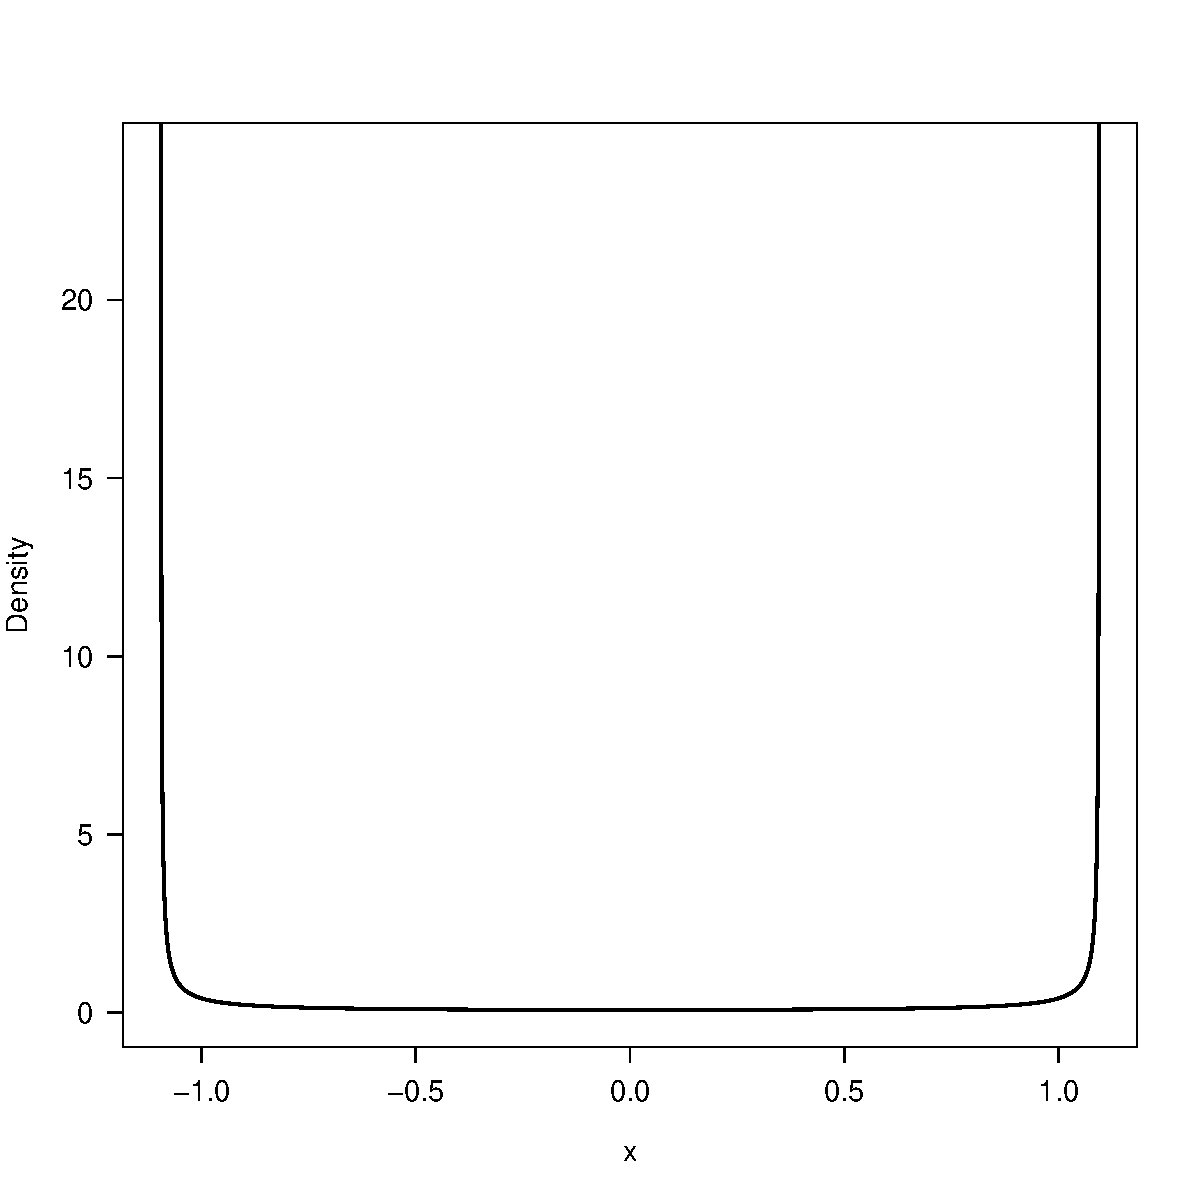
\includegraphics[width=0.46\textwidth]{chunks/beta}}
	\subfigure[Gamma distribution]{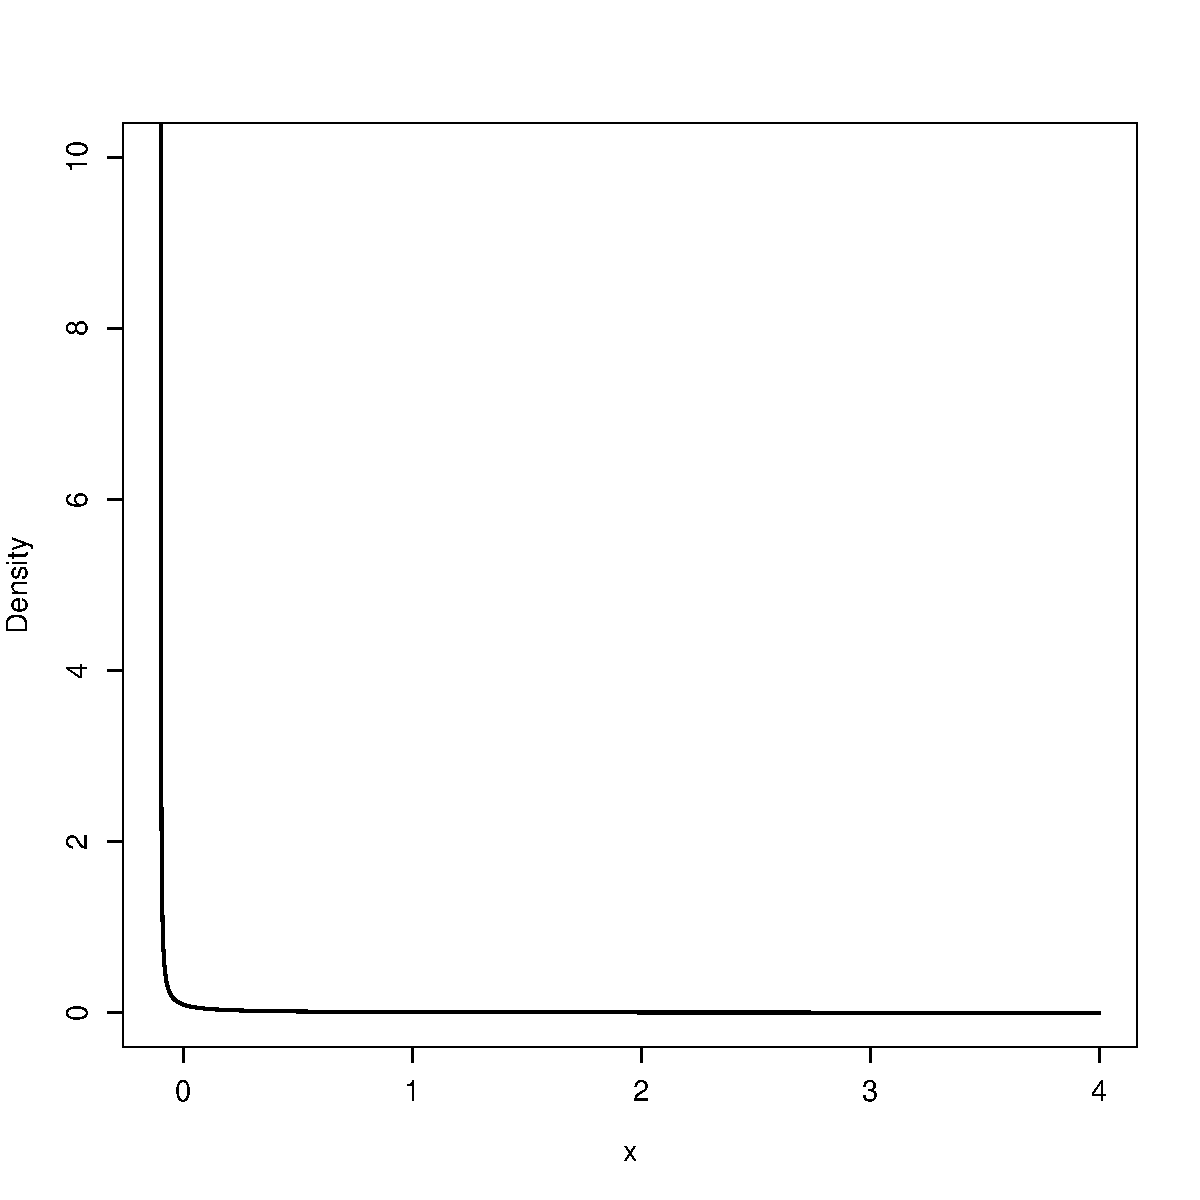
\includegraphics[width=0.46\textwidth]{chunks/gamma}}
	\caption{Rescaled $\textrm{Beta}(1/10, 1/10)$ and $\textrm{Gamma}(1/100, 1/100)$ distributions with variance $1$ and mean $0$.}
	\label{fig::distributions}
\end{figure}

\item Scaled and centered Beta distribution with $\alpha=\beta=1/10$. This is a bimodal distribution with a lot of weight placed on the modes. See the left of Figure \ref{fig::distributions}.
\item Scaled and centered Gamma distribution with $\alpha=\beta=1/100$. This is asymmetric and with heavy tails. See the right of Figure \ref{fig::distributions}.
\end{enumerate}

I have chosen $5$ degrees of freedom for the $t$-distribution since it is the first integer degree of freedom where $t$ has finite fourth moment. The parameters for the Beta and Gamma make them both extreme, as should be clear from Figure \ref{fig::distributions}. I have chosen these distributions since they are extreme and should be able to force out some difference between the estimators. The Open Science Foundation repository for this paper (\url{https://osf.io/s356h/}) contains the code I used to run the simulations.

Table \ref{tab:simulation} contains $100 \times \MSE_\alpha/\MSE_{\alpha_S}$, where $\MSE$ denotes the mean squared error. Values higher than $100$ are in favor of $\hat{\alpha}_s$ and values lower than $100$ in favor of $\hat{\alpha}$. The table shows that $\alpha_S$ tends to outperform $\alpha$ when both $k$ and $n$ is large and $\sigma$ is small, but with no clear trends otherwise. In this simulation $\hat{\alpha}_s$ does slightly better than $\hat{\alpha}$ -- the geometric mean of $\MSE_\alpha/\MSE_{\alpha_S}$ is $1.08$, giving an $8$\% advantage to $\hat{\alpha}_s$. Of course, this is a small simulation study and it is hard to predict what would happen with other distributions. Still, I believe the result of these simulations should be counted in favor of sample standardized alpha.

To sum up, sample alpha won the maximum likelihood and robustness competitions, drew the asymptotic efficiency competition, and lost the finite sample competition. The tally is sample alpha 2\sfrac{1}{2} - 1\sfrac{1}{2} standardized alpha. 

%% <<<<< Example table start (\label{tab:reliabilites})
% latex table generated in R 3.6.2 by xtable 1.8-4 package
% Mon Feb 03 15:19:37 2020
\begin{table}[ht]
\centering
\caption{Simulations of $100 \times \textrm{MSE}_\alpha/\textrm{MSE}_{\alpha_s}$ in the parallel model} 
\begin{tabular}{rlllllllll}
    & $t(5)$ & $t(5)$ & $t(5)$ & Beta & Beta & Beta & Gamma & Gamma & Gamma \\
  & $\sigma = 2$ & $\sigma = 1$ & $\sigma = 0.5$ & $\sigma = 2$ & $\sigma = 1$ & $\sigma = 0.5$ & $\sigma = 2$ & $\sigma = 1$ & $\sigma = 0.5$ \\
$k = 5, n = 50$ & 106 & 112 & 103 & 106 & 112 & 114 & 107 & 105 & 113 \\ 
  $k = 20, n = 50$ & 113 & 105 & 105 & 95.8 & 90.8 & 98.9 & 97.5 & 97.6 & 94.7 \\ 
  $k = 5, n = 200$ & 99.5 & 98.7 & 102 & 101 & 101 & 100 & 74.7 & 60.6 & 67.4 \\ 
  $k = 20, n = 200$ & 37.8 & 174 & 138 & 144 & 82.6 & 308 & 257 & 189 & 153 \\ 
  \end{tabular}
\end{table}
\newcommand{\geomean}{1.08}


%% example table end >>>>>

\section{Argument B. The problem with standardized scores}
\label{sec:argument B}
I have two arguments against using standardized alpha for standardized
test items. First, you should not standardize test items. Second,
even if you decide to standardize test items, avoid standardized
alpha and use the standardized reliability instead.

Before I begin fleshing out these arguments, I will explain why standardized alpha is explicitly linked to the standardized scores $w_i = {(\lambda_i^2 + \sigma_i^2)}^{1/2}$,  but not to the unit scores. My starting point is the following claim of \citet[][p.348]{Osburn2000-jd}: 
\enquote{[] it is important to note that the true reliability of a measure is the same for both standardized and unstandardized observed scores.}

I will argue against this claim. Recall the definition of reliability from
section $2$. Given a predictor $\hat{Z}$ of $Z$, the
reliability $\omega$ equals the square correlation between $\hat{Z}$
and $Z$, or $\omega=\Cor^{2}(\hat{Z},Z)$. Assume
we know the values of $\lambda$ and $\sigma$. When you use unstandardized
scores, your predictor is $$\hat{Z}=w_{0}\sum_{i=1}^{k}X_{i}$$
where $w_{0}=\overline{\lambda}/(k\overline{\lambda}^{2}+\overline{\sigma^{2}})$ scales the predictions to match $\Var Z=1$ (Proposition \ref{prop:reliability motivation}). When you use standardized
scores, your predictor is $$
\hat{Z}^{*}=w_{0}\sum_{i=1}^{k}(\lambda^{2}+\sigma^{2})^{-1/2}X_{i}.$$
These predictors are not the same in general, and their reliabilities are not
the same either.

This difference matters. Reliability coefficients are useful because they tell you how good you can expected your prediction of $Z$ based on $X$ to be. Provided you use the mean squared error as a measure of prediction success, this is exactly what the equivalent reliability concept in Proposition \ref{prop:reliability motivation} says. For $1 - \MSE(w_0\hat{Z})$ puts a number between $0$ and $1$ on the expected quality of your prediction. If you do not use $\hat{Z}$, but some other predictor $\hat{Z}'$, this concrete interpretation of the reliability disappears. 

An important motivation for using the squared
correlation between $Z$ and $\hat{Z}$ as the definition of a
reliability coefficient is that it allows us to do correction for
attenuation. Let $\hat{Z}_{1},\hat{Z}_{2}$ be two linear
predictors of two latent variables $Z_{1},Z_{2}$ defined in two separate
congeneric models. Assume the errors $\varepsilon_{1}$ and $\varepsilon_{2}$ of these models
are uncorrelated. Our goal is to find the correlation $\Cor(Z_{1},Z_{2})$
between the latent variables $Z_{1}$ and $Z_{2}$ using only the
reliabilities $\omega(\hat{Z}_{1})$, $\omega(\hat{Z}_{2})$,
and the observed correlation $\Cor(\hat{Z}_{1},\hat{Z}_{2})$.
Then
\begin{eqnarray*}
\Cor(\hat{Z}_{1},\hat{Z}_{2}) & = & \frac{\Cov(Z_{1},\hat{Z}_{1})\Cov(Z_{2},\hat{Z}_{2})}{\sd(\hat{Z}_{1})\sd(\hat{Z}_{2})}\Cor(Z_{1},Z_{2})\\
 & = & \omega(\hat{Z}_{1})\omega(\hat{Z}_{2})\Cor(Z_{1},Z_{2})
\end{eqnarray*}
and $\Cor(Z_{1},Z_{2})=\Cor(\hat{Z}_{1},\hat{Z}_{2})/[\omega(\hat{Z}_{1})\omega(\hat{Z}_{2})]$,
the famous Spearman \citet{spearman1904proof} attenuation formula.

But correction for attenuation cannot be used unless both $\omega(\hat{Z}_i)$s are the squared correlation between $\hat{Z}_i$ and $Z_i$. For example, if you used the standardized sum scores to make predictions for the first model, it would be wrong to use the congeneric reliability, as it based on the sum scores. If you used the congeneric reliability, the correlation between $Z_1$ and $Z_2$ would incorrectly be calculated according to $$\rho'=\omega(\hat{Z}_{1})\omega(\hat{Z}_{2})\Cor(Z_{1},Z_{2})$$
instead of the correct $\rho=\omega(\hat{Z}_{1}^{*})\omega(\hat{Z}_{2})\Cor(Z_{1},Z_{2})$.
You would be off by a factor of $\omega(\hat{Z}_{1}^{*})/\omega(\hat{Z}_{1})$.

This connection between reliabilities and the choice of predictor
weights is not new. It has been observed by e.g. \citet[][p. 112]{Joreskog1971-nn} and \citet{McNeish2018-vu}, who repeatedly insists on taking this connection into account. Several authors recommend you use standardized alpha with standardized sum scores. For instance, \citet[][p. 451]{Falk2011-ae} states \enquote{If researchers intend to sum
standardized scores, the correlation matrix is more appropriate for determining internal consistency,} while \citet[][p. 99]{Cortina1993-aq} says \enquote{Standardized alpha is appropriate if item standard scores are summed to form scale scores.}

You should never standardized your items. That is, you should avoid $w_{i}=(\lambda_{i}^{2}+\sigma_{i}^{2})^{-1/2}$ when you form your linear predictor.
Using some $w\ne1$ seems reasonable, for you would not want items
with large variance to overshadow all the other contributions to $\hat{Z}$.
But there is something strange about this particular $w$. Dividing by $(\sigma_{i}^{2}+\lambda_{i}^{2})^{1/2}$
seems wrong, as you want items with large loadings, i.e., $\lambda_{i}$s, to have a large
influence on your prediction of $Z$. But dividing by $(\sigma_{i}^{2}+\lambda_{i}^{2})^{1/2}$
makes the influence of items with large loadings smaller!

The weights $w_i=\sigma_{i}^{-1}$ is an intuitive alternative to standardized weights. These weights make the contribution of each $\lambda_i$ directly comparable, as the modified model $wX$ will have all residual standard deviations equal to $1$ and factor loadings equal to the standardized factor loadings $\lambda_i/\sigma_i$. Since the weights do not involve $\lambda$, they do not penalize items with large loadings. 

Call the reliability with weights $w=\sigma^{-1}$ the \textit{sigma reliability} and denote it $\omega_\sigma$. Using Proposition \ref{prop:reliability motivation}, it can be written as
\begin{equation}
\omega_\sigma=\frac{k\overline{\lambda\sigma^{-1}}^{2}}{k\overline{\lambda\sigma^{-1}}^{2}+1}.\label{eq:Sigma-standardized reliability}
\end{equation}

Another option is to use the optimal weights, yielding coefficient $H$ and the Thurstone factor scores instead of the standardized alpha and standardized sum scores.  \citet{McNeish2019-ea} argue in favour of adopting optimal weights when forming the predictor. 

The following theorem exposes some basic facts about these four reliability coefficients.

\begin{thm}
\label{thm:Properties of three} Let $\omega$ be the congeneric
reliability \eqref{eq:Congeneric reliability}, $\omega_{s}$ the standardized reliability \eqref{eq:Standardized reliability},
$\omega_{\sigma}$ the sigma reliability \eqref{eq:Sigma-standardized reliability},
and $\omega_{H}$ coefficient $H$ \eqref{eq:coefficient_H}. 

\begin{enumerate}[label=(\roman*)]
\item Assume the $\tau$-equivalent model,
i.e. the congeneric model with $\lambda_{i}=\lambda>0$ for all $i$
but possibly different residual errors $\sigma_{i}>0$. Then
\[
\omega_{h}\geq\omega_{\sigma}\geq\omega_{s}\geq\omega,
\]
with all inequalities strict unless $\sigma_{i}=\sigma$ for all
$i$. In that case, $\omega_{h} = \omega_{\sigma} = \omega_{s} = \omega$.
\item Assume the congeneric model with $\sigma_i = \sigma > 0$ for all $i$ but possibly different loadings $\lambda_i$. Then
\[
\omega_{H}\geq\omega_{\sigma}=\omega\geq\omega_{s},
\]
and the inequalities are strict unless $\lambda_{i}=\lambda$ for all
$i$. In that case, $\omega_{h} = \omega_{\sigma} = \omega_{s} = \omega$.

\end{enumerate}

\end{thm}
\begin{proof}
See the appendix, page \pageref{proof:Properties}.
\end{proof}

Since the $\tau$-equivalent model is such a common assumption among psychometricians, point (i) of the theorem above gives a strong reason to prefer $\omega_{\sigma}$ to $\omega_s$ and $\omega$. Point (ii) can be used as an argument against using the standardized reliability \eqref{eq:Standardized reliability} when $\sigma_{i}^{2}=\sigma_j^{2}$ for all $i,j$.

You can interpret Theorem \ref{thm:Properties of three} as a ranking factor scores too. Under the $\tau$-equivalent model, Thurstone scores are better than $\sigma$-standardized sum scores, which in turn are better than the standardized sum scores, which are
better than the ordinary sum scores.

Theorem \ref{thm:Properties of three} shows how the four reliabilities relate to each other only under the $\tau$-equivalent model and the model where all $\sigma_i$s are equal. If we assume only the congeneric model, the nice inequalities of Theorem \ref{thm:Properties of three} disappear. Since coefficient $H$ uses the optimal weights, it is guaranteed to be larger than the three other reliabilities mentioned above. The
other three reliabilities can be in any order, but
$\omega_{\sigma}$ will usually be the largest. In a short
simulation ($10^{5}$ repetitions) of $k=5$ items with $\lambda_{i}\sim \textrm{Exp}(1)$
and $\sigma_{i}\sim \textrm{Exp}(1)$ independently with $i=1,\ldots,5$, $\omega_{\sigma}$
was the largest $98\%$ of the time, $\omega$ largest $2\%$
of the time, but $\omega_{s}$ was never the largest. The average reliabilities where $\overline{\omega}_\sigma = 0.91$, $\overline{\omega}_s= 0.76$, and $\overline{\omega} = 0.70$.
The congeneric reliability $\omega$ dominated the standardized $\omega_{s}$ in $4/10$ iterations. You could argue this simulation study
is somewhat unrealistic, but the slightly different simulation with $\lambda_{i}$ and $\sigma_{i}\sim \textrm{HalfNormal}(0,1)$, yielded virtually the same results. In a simulation where $\lambda$ and $\sigma$ where uniform on $[0,1]$, yet again $\omega_{\sigma}$
was the largest $98\%$ of the time and $\omega$ the largest the remaining $2\%$. Moreover, in every iteration of every simulations $\omega_\sigma > \omega_s$. The take-away message from these simulations is that $\omega_\sigma$ generally does better than $\omega_{s}$ and
$\omega$, while it is hard to predict the winner among $\omega$
and $\omega_{s}$. See the Open Science Foundation repository for this paper (\url{https://osf.io/s356h/}) for the code to run these informal simulations.

\begin{example}
\label{exa:reliabilities}
%% <<<<< Example table start (\label{tab:reliabilites})
% latex table generated in R 4.0.0 by xtable 1.8-4 package
% Thu May 14 11:11:44 2020
\begin{table}[ht]
\centering
\caption{Comparison of reliability coefficients on personality data} 
\label{tab:reliabilites}
\begin{tabular}{lccccc}
  \toprule
 & A & C & E & N & O \\ 
  \cmidrule{1-6}
Congeneric reliability ($R$) & 0.712 & 0.733 & 0.767 & 0.813 & 0.610 \\ 
  Coefficient \it{H} ($R_H$) & 0.765 & 0.739 & 0.778 & 0.850 & 0.651 \\ 
  Standardized reliability ($R_S$) & 0.724 & 0.734 & 0.763 & 0.815 & 0.618 \\ 
  Sigma reliability ($R_\sigma$) & 0.744 & 0.736 & 0.770 & 0.836 & 0.630 \\ 
   \bottomrule
\end{tabular}
  \vskip7.0pt
A, agreeableness; C, conscientiousness; E, extraversion; N, neuroticism; O, openness to experience 
\end{table}

%% example table end >>>>>

In this example we will take a look at the data set $\texttt{bfi}$ from he $\texttt{R}$ \citep{Team2013-tt} package $\texttt{psychTools}$ \citep{Revelle2019-te}. This data set contains the responses on $25$ personality self report items from the International Personality Item Pool \citep{Goldberg1999-iz} collected from the Synthetic Aperture Personality Assessment project \citep{Revelle2017-ez}. The $25$ items are evenly distributed across the big five traits: Agreeableness, conscientiousness, extraversion, neuroticism, and openness to experience. 

For each trait I estimated the factor loadings $\lambda$ and residual standard deviations $\sigma$ in the congeneric measurement model \eqref{eq:congeneric model} using  $\texttt{lavaan}$ \citep{Rosseel2012-yg}. I plugged these estimates into the definitions of the four reliability coefficients. The results are in Table \ref{tab:reliabilites}. As expected, $\omega_\sigma$ is larger than both $\omega_s$ and $\omega$ for all five traits. Moreover, $\omega_s > \omega$ for all traits except extraversion, where the difference is marginal. The Open Science Foundation repository for this paper (\url{https://osf.io/s356h/}) contains the code I used in this example.
\end{example} 

Suppose you want to use the standardized weights despite the counterarguments above. By Proposition \ref{prop:weighted alpha}, the standardized coefficient alpha equals the standardized reliability only when the modified model
\begin{equation}\label{eq:std-modified model}
X_{i}^{*}=\frac{\lambda_{i}}{\sqrt{\lambda_{i}^{2}+\sigma_{i}^{2}}}Z+\frac{\sigma_{i}}{\sqrt{\lambda_{i}^{2}+\sigma_{i}^{2}}}\varepsilon_{i}\:i=1,\ldots,k    \end{equation}
is $\tau$-equivalent. This occurs if and only if each $\lambda_{i}/(\lambda_{i}^{2}+\sigma_{i}^{2})=\lambda^{*}$
for some $\lambda^{*}$. Of course, this would be an exceptional coincidence, but the standardized alpha is just a lower bound for the true standardized reliability when this condition fails. The natural way to estimate $\omega_w$ consistently without making this unwarranted assumption, use the plug-in estimator for $\omega_s$ \eqref{eq:Standardized reliability}. This is not hard, as estimation of $\lambda_{i},\sigma_{i}$ with structural equation modeling programs is routine.

\begin{example}
%% <<<<< Example table start (\label{tab:omega_std_alpha_std})
%% latex table generated in R 3.6.2 by xtable 1.8-4 package
% Wed Feb 26 15:09:33 2020
\begin{table}[ht]
\centering
\begin{tabular}{rllll}
   \multicolumn{5}{c}{Mean squared error times $n$}\tabularnewline 
 & $n = 50$ & $n = 200$ & $n = 1000$ & $n = 5000$ \\ 
 $\omega_s$ & 0.19 & 0.18 & 0.17 & 0.18 \\ 
  $\alpha_s$ & 4.8 &  15 &  74 & 365 \\ 
   \multicolumn{5}{c}{Bias}\tabularnewline \\ 
 & $n = 50$ & $n = 200 & $n = 1000$ & $n = 5000$ 
 $\$\omega_s$_s$ & -0.0028 & 0.00016 & -0.00099 & -0.00025 \\ 
  $\$\alpha_s$_s$ & -0.29 & -0.27 & -0.27 & -0.27 \\ 
  \end{tabular}
\end{table}

%% example table end >>>>>
I used $\mathtt{lavaan}$ to estimate $\lambda$ and $\sigma$ for the agreeableness factor on the the $\texttt{bfi}$ data from $\texttt{psychTools}$ \citep{Revelle2019-te}, the data used in Example \ref{exa:reliabilities}. The estimates are $\hat{\lambda} = (0.53, -0.77, -0.99, -0.72, -0.79)$ and $\hat{\sigma} = (1.3, 0.89, 0.85, 1.3, 0.98)$. Using formula \eqref{eq:standardized alpha} and \eqref{eq:Standardized reliability} and flipping the sign of reverse-scored item \eqref{eq:Standardized reliability}, we find $\hat{\omega}_s = 0.72$ and $\hat{\alpha}_s = 0.71$. The difference $\hat{\alpha}_s - \hat{\omega}_s = -0.011$ is not alarmingly high, but the estimator is inconsistent. Table \ref{tab:reliabilites} contains mean squared error calculations for different $n$s when with data simulated from a congeneric model with $\lambda=\hat{\lambda}$ and $\sigma = \hat{\sigma}$. The mean squared error is uniformly lower for $\hat{\omega}_s$ than $\hat{\alpha}_s$. The results are similar for the other traits in the $\texttt{bfi}$ data.
\end{example}

To recap, my arguments are: (i) You should neither avoid standardization altogether nor standardize with $(\lambda_{i}^{2}+\sigma_{i}^{2})^{-1/2}$. You should standardize with $\sigma_i^{-1}$ or use the optimal weights, as this yields better results in the most plausible scenarios. (ii) Even if you decide to standardize with $(\lambda_{i}^{2}+\sigma_{i}^{2})^{-1/2}$, please avoid standardized alpha, as won't equal $\omega_s$ under any reasonable assumptions.

\section{Ordinal alpha\label{sec:Ordinal alpha}}

Recall the congeneric model
\begin{equation}
X=\lambda Z+\Psi^{1/2}\varepsilon    \tag{\ref{eq:congeneric model}}
\end{equation}
Consider the scenario when we do not observe the $X_{i}$s directly,
but rather $X_{i}$s discretized into $m_{i}$ categories according
to
\begin{equation}
Y_{i}=k1[\tau_{i(k-1)}\leq X_{i}\leq\tau_{ik}],\label{eq:discretization model}
\end{equation}
where $-\infty=\tau_{i0}<\tau_{i1}<\ldots<\tau_{i(m_{i}+1)}=\infty$
are thresholds for each $i$ and $1[A]$ is the indicator function of $A$.
This is a common model for Likert scales with $m_{i}$ levels for
the $i$th item. If $X$ is multivariate normal, model (\ref{eq:discretization model})
is a congeneric \emph{ogive model} \citep{Swaminathan2016-rg}.
Under multivariate normality the correlation matrix $\Phi$ is point-identified
from the distribution of $Y$, and is called the \emph{polychoric
correlation}. It can be estimated by maximum likelihood directly
or by a two-step procedure \citep{Olsson1979-ti}. To make the model
identified, usual practice is to assume that $\Psi^{1/2}$ is correlation
matrix. 

\citet{Zumbo2007-ap} proposed what I call the \emph{theoretical ordinal
alpha}
\begin{equation}
\alpha=\frac{k}{k-1}\left(1-\frac{k}{\mathbf{i}^{T}\Phi\mathbf{i}}\right)\label{eq:ordinal alpha}
\end{equation}
where $\Phi=\Cor X$ is polychoric correlation coefficient of $Y$.
Theoretical ordinal alpha is a standardized alpha, but it is based
on the latent correlation matrix between the unobserved $X$ instead
of the observed correlation matrix between the $Y$s. The population
values of the theoretical ordinal alpha and the standardized alpha
are not the same in general. \citet{Zumbo2007-ap}'s main argument
in favor of the ordinal alpha is ``coefficient alpha (and KR-20)
are correlation-based statistics and hence assume continuous data\textquoteright \textquoteright{}
\citep[p. 27]{Zumbo2007-ap}. In section \ref{sec:coefficienta alpha} I argued against the notion that coefficient alpha only makes sense for continuous data. \citet[p. 1060, "Misconception 1"]{Chalmers2018-fj}
persuasively argues against this idea, see also \citep{Raykov2019-yr}. The argument is reiterated
by \citep{Gadermann2012-jl}, but \citet{Zumbo2019-lm} argue
the the benefit of sample ordinal alpha is that we are truly interested
in the reliability of $X$ as a predictor of $Y$ (in the parlance
of this paper). 

A related notion is the \emph{theoretical ordinal reliability}, the
analogue of the weighted reliability \eqref{eq:linear reliabiltiy} based on the polychoric
correlation coefficient. Its definition is 
\begin{equation}
\omega_{w}=\frac{w\lambda_{i}^{*}}{w\lambda_{i}^{*}+\sigma_{i}^{*}}\label{eq:ordinal omega}
\end{equation}
were $\lambda_{i}^{*}=\lambda_{i}/\sqrt{\lambda_{i}^{2}+\sigma_{i}^{2}}$
and $\sigma_{i}^{*}=\sigma_{i}/\sqrt{\lambda_{i}^{2}+\sigma_{i}^{2}}$.

There several reasons to avoid the theoretical ordinal alpha. If your
goal is to estimate the congeneric reliability or the standardized
reliability, the theoretical ordinal alpha is inappropriate since
it does not equal the congeneric reliability, even under the parallel
model \citep[p. 1062, "Misconception 2"]{Chalmers2018-fj}, a point
conceded by \citet{Zumbo2019-lm}. But this is not the worst problem.
For even if you are interested in estimating the congeneric reliability
for the multivariate normal ogive model, you should avoid the theoretical
alpha.

Theoretical ordinal alpha is apparently not connected to any predictor
of $Z$ that depends on the data $Y$, only the squared correlation $\Cor^{2}(\hat{Z},Z)$ where $\hat{Z}=\sum_{i=1}^k w_iX_i$. This correlation is barely interesting though, as we do not observe
the latent $X_{i}$s. The theoretical alpha does not have the concrete
interpretation of the congeneric alpha mentioned in section 2. The question
``how good can I expected my prediction of $Z$ based on $X$ to
be?'' does not make practical sense to ask, as $X$ is unknown and you cannot use it for your prediction. This
lack of knowledge about $X$ also makes correction for attenuation
impossible. Since $X$ is unknown, it is impossible to directly calculate
the correlation between a function of $X$ and a function of some
other quantity $X'$. Due to this, the correction for attenuation formula
will not work. 

Moreover, if you want the standardized reliability of the unobserved
$X$, the ordinal reliability is a better choice. For the conditions
required for standardized alpha to equal the standardized reliability
are still needed, i.e. the weighted $\tau$-equivalent model \eqref{eq:std-modified model}. The
theoretical ordinal reliability can be estimated using e.g. $\mathtt{lavaan}$
without much added complexity. Using the same arguments as in the
previous section, the theoretical ordinal reliability with optimal
weights (corresponding to coefficient \emph{H}) or weights $w_{i}=\sigma_{i}$
(corresponding to the sigma reliability) should be preferred to the
standardized reliability too.

Finally, theoretical ordinal alpha only makes sense in relation to
the congeneric multivariate ogive model. But this model depends on
the fundamentally unverifiable assumption of multivariate normality
of $X$. The polychoric correlation coefficient is not robust against
normality in general \citep{Foldnes2019-yd}. 

\subsection{A concrete ordinal reliability}

The main argument of \citet{Zumbo2019-lm}'s rebuttal of \citep{Chalmers2018-fj}
is that the congeneric ogive model \eqref{eq:discretization model} 
is a better approximation to reality than the congeneric model \eqref{eq:congeneric model}. (See also \citet[][p.2]{Gadermann2012-jl}.)
So assume we believe in the discretized model and can be reasonably
sure that $X$ is multivariate normal. Then ordinal alpha would still
not be appropriate as it is theoretical and not concrete. However,
it is possible to create a class of reliability coefficients for the
congeneric ogive model.

Let $\hat{X}_{i}$ be the mean of a standard normal distribution
truncated to $(\tau_{i(Y_{i}-1)},\tau_{iY_{i}}]$, or equivalently
\begin{equation}
\hat{X}_{i}=-\frac{\phi(\tau_{iY_{i}})-\phi(\tau_{i(Y_{i}-1)})}{\Phi(\tau_{iY_{i}})-\Phi(\tau_{i(Y_{i}-1)})},\label{eq:Predictor of X}
\end{equation}
see \citep[Section 10.1]{Johnson1994-ag} for the formula for the
expectation of a truncated normal. Since $\hat{X}_{i}$ is the
conditional expectation of $X_{i}$ given $Y_{i}$, it is the optimal
predictor of $X_{i}$ given $Y_{i}$ in the sense of minimizing the
mean squared error. A natural predictor of $Z$ given $Y$ is a linear
function of $\hat{X}_{i}$, i.e. $\hat{Z} = \sum_{i=1}^{k}w_{i}\hat{X}_{i}$
for some weights $w_{i}$, which gives rise to the analogue of the
weighted reliability \eqref{eq:linear reliabiltiy} in the context of the congeneric ogive model
(\ref{eq:discretization model}) when $X$ is multivariate normal
with standard normal marginals. 
\begin{defn}\label{defn:weighted ordinal reliability}
Let $w$ be a vector of weights and $\hat{Z}=\sum_{i=1}^{k}w_{i}\hat{X}_{i}$, with $\hat{X}_i$ as in \eqref{eq:Predictor of X}. The \textit{weighted ordinal} reliability is $\omega_{w}'=\Cor^2(\hat{Z},Z)$.
\end{defn}
The following theorem shows how to calculate $\omega_{w}'$ and
some of its properties.
\begin{thm}
\label{thm:omega-prime}Let $\hat{Z}=\sum_{i=1}^{k}w_{i}\hat{X}_{i}$
with $\hat{X}$ defined as in \eqref{eq:Predictor of X} and $\Xi=\Cov\hat{X}$.
Assume $X$ is multivariate normal with standard normal marginals,
such that $\sqrt{\lambda_{i}^{2}+\sigma_{i}^{2}}=1$ for all $i$.
\begin{enumerate}[label=(\roman*)]
\item Let  $v_{i}=\lambda_{i}/[\sigma_{i}^{2}(1+k\overline{\lambda^{2}\sigma^{-2}})],\:i=1,\ldots,k$ be the Thurstone weights. Then $\sum_{i=1}^{k}v_{i}\hat{X}_{i}$
is the optimal predictor of $Z$, i.e. it minimizes the mean squared
error $\MSE(\hat{Z})$.
\item The weighted ordinal reliability is
\begin{eqnarray}
\omega_{w}' & = & \frac{(w^{T}\Xi v)^{2}}{w^{T}\Xi w}\label{eq:Omega prime}\\
 & = & 1-\MSE(v_{0}\hat{Z})\nonumber 
\end{eqnarray}
where $v_{i}=\lambda_{i}/[\sigma_{i}^{2}(1+k\overline{\lambda^{2}\sigma^{-2}})],\:i=1,\ldots,k$
are the Thurstone weights for $X$ and $v_{0}=w^{T}\Xi v$ is the
minimizer of $\MSE(v_{0}\hat{Z})$. Moreover, $\omega_{v}'=v^{T}\Xi v$ when $v$
are the Thurstone weights.
\item When the underlying congeneric model is parallel and $w=\mathbf{i}$,
\begin{eqnarray}
\omega_{w}' & = & \frac{\lambda^{2}}{(k\lambda^{2}+\sigma^{2})^{2}}\mathbf{i}^{T}\Xi\mathbf{i},\label{eq:Alpha prime}\\
 & = & \alpha_S\frac{\mathbf{i}^{T}\Xi\mathbf{i}}{\mathbf{i}^{T}\Psi\mathbf{i}},\nonumber 
\end{eqnarray}
where $\alpha_S$ equals the ordinal alpha.
\item For any weight $w$, $\omega'_{w}\to\omega_{w}$ when $\Xi\to\Phi$. 
\end{enumerate}
\end{thm}

\begin{proof}
See the appendix, page \pageref{proof:omega-prime}.
\end{proof}
Point (i) is a strong justification for using $\hat{Z}=\sum_{i=1}^{k}v_{i}\hat{X}_{i}$,
where $v_{i}$ are the Thurstone weights. This is not only the optimal
linear predictor of $Z$ given the data $Y$, it is the optimal predictor
of $Z$ period. The analogous result for the congeneric model with
multivariate normal $X$ is also true, that is, $Z=\sum_{i=1}^{k}v_{i}X_{i}$
is the optimal predictor of $Z$. (This follows from the proof of
Theorem \pageref{thm:omega-prime}.) The representation of the ordinal
reliability in (ii) is similar to the representation of the weighted
reliability in Proposition \ref{prop:reliability motivation}, but the covariance $\Xi$ is used
instead of $\Sigma$. Moreover, $v^{T}\Xi v$ is easy to estimate
provided we are able to estimate the Thurstone weights $v$. 

Point (iii) demonstrates that $\omega'$ with unit weights can be
calculated without running a factor analysis, since the average correlation
$\mathbf{i}^{T}\Xi\mathbf{i}/\mathbf{i}^{T}\Psi\mathbf{i}$ is a simple
function of the polychoric correlation matrix and the covariance matrix
of $\hat{X}.$ Moreover, $\alpha_S(\mathbf{i}^{T}\Xi\mathbf{i}/\mathbf{i}^{T}\Psi\mathbf{i})$
is the natural variant of the standardized alpha in the ordinal setting,
as it is defined in terms of the matrices $\Xi$ and $\Psi$ only,
and is designed to equal the ordinal reliability under the parallel
model. 

\citet[p. 1068]{Chalmers2018-fj} discusses one possible use of the
ordinal alpha, namely as the theoretical reliability when the number
of thresholds $\tau$ goes towards infinity. Point (iv) makes this
claim concrete.

\begin{example}
We will yet again have a look at $6$-level agreeableness factor the
personally data $\mathtt{bfi}$ from $\mathtt{psychTools}$. I did the calculations in this example with the $\mathtt{conogive}$ package \citep{conogive}. This package employs the $\mathtt{psych}$ \citep{psych} package to fit the congeneric ogive
model \eqref{eq:discretization model} using the two-step procedure
to estimate the polychoric correlation matrix, and then calls the $\mathtt{fa}$ function to run a factor analysis on the said matrix.
The resulting estimates are 
\begin{eqnarray*}
\hat{\lambda} & = & (0.43,0.71,0.80,0.52,0.67),\\
\hat{\sigma} & = & (0.90,0.70,0.59,0.86,0.74).
\end{eqnarray*} The ordinal reliability
with optimal weights is $\omega'_{H}=0.68$, and with equal weights
and $\omega'=0.64$. But the theoretical variants are $\omega'_{H}=0.81$
and $\omega'=0.77$, both missed by large margin. In comparison, the
reliabilities calculated under the congeneric model with $\mathtt{lavaan}$ \citep{Rosseel2012-yg}
equals $\omega'_{H}=0.77$ and $\omega'=0.74$.

I calculated $\omega'_{H}$ and $\omega'$ for selection of Likert
scales with $\lambda=\hat{\lambda}$ and $\hat{\sigma}=\sigma$ and
the thresholds $\tau$ at $\{\Phi^{-1}[i/(k+1)]\}_{i=1}^{k+1}$, which
approximates the reliabilities we would have obtained had we used
$k+1$ Likert levels. Figure \ref{fig:Ordinal reliability} contains the results. The difference between ordinal alpha and the true ordinal reliability is uniformly at approximately $0.04$. The distance from theoretical ordinal reliability to actual ordinal reliability is larger than $0.04$ when the number of Likert levels is less than $10$, and unacceptably large when the number of Likert levels is less than $6$. 
\end{example}

\begin{figure}
\noindent \begin{centering}
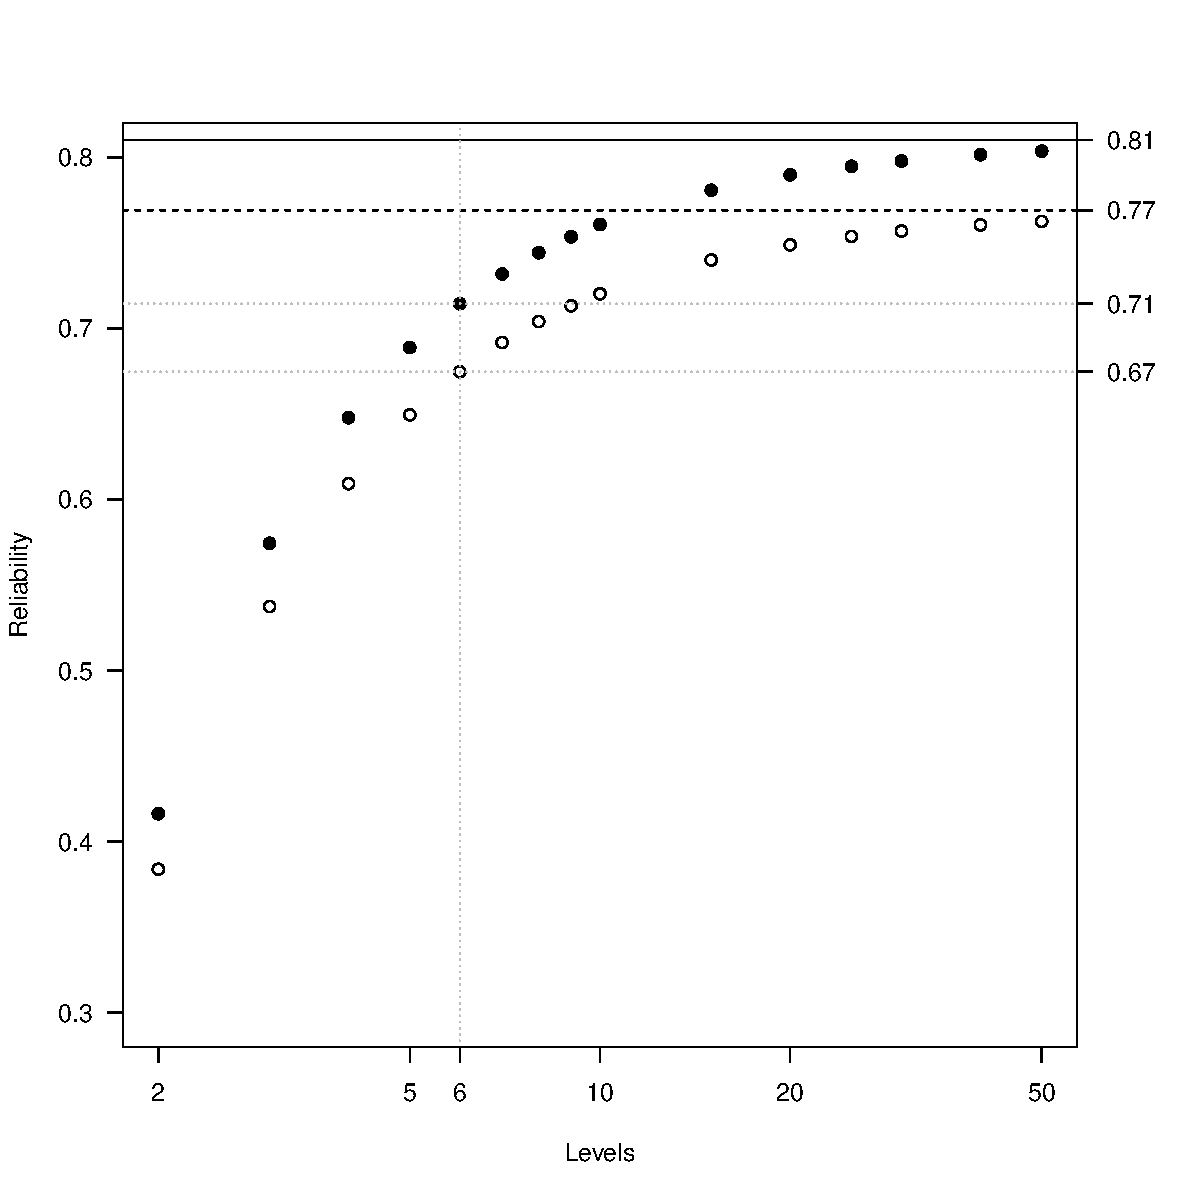
\includegraphics[scale=0.5]{chunks/ordinals}
\par\end{centering}
\caption{\label{fig:Ordinal reliability}Ordinal reliability ($\fullmoon$)
and ordinal $H$ ($\newmoon$) for a selection of Likert levels. The
theoretical coefficient $H$ is $0.81$ (solid line), and the theoretical
composite reliability is $0.77$ (dashed line). All cutoffs are uniform,
and every reliability has been calculated with $\lambda=(0.43,0.71,0.80,0.52,0.67)$
and $\sigma=(0.90,0.70,0.59,0.86,0.74)$. The original number of levels
($6$) and the ordinal reliabilities $(\omega'_{H}=0.71,\omega'=0.67)$
are marked for convenience.}
\end{figure}

\section*{Appendix}

This lemma formulates the the squared correlation in terms of the mean squared error and established the connection between the correlation coefficient and $R^2$. It is used in in the proof of Proposition \ref{prop:reliability motivation}. 
\begin{lem}
\label{lem:r^2 and correlation}Assume $Y$ and $\hat{Y}$ have finite
variance. If $Z$ is a random variable, let $\MSE(Z) = E[(X-Z)^2]$ denote the mean squared error of $Z$ as predictor of $X$. Then 
\begin{equation}
\Cor^{2}(\hat{Y},Y)=1-\frac{\MSE(\alpha+\beta\hat{Y})}{\Var(Y)},\label{eq:rsq and correlation}
\end{equation}
where $\alpha=E(Y)-E(\hat{Y})$ and $\beta=\Cov(\hat{Y},Y)/\Var(\hat{Y})$ are the theoretical regression coefficients minimizing the mean squared error $\MSE(\alpha+\beta\hat{Y})$. 
\end{lem}

\begin{proof}
Recenter $Y$ and $\hat{Y}$ so that $E(Y)=E(\hat{Y})=0$. Then $\MSE(\alpha+\beta\hat{Y})$ equals $\beta^{2}\Var(\hat{Y})-2\beta\Cov(\hat{Y},Y)+\Var Y^{2}$.
Differentiate with respect to $\beta$ and set equal to zero, so that
$2\beta\Var(\hat{Y})-2\Cov(\hat{Y},Y)=0$. Then $\beta=\Cov(\hat{Y},Y)/\Var(\hat{Y})$
\end{proof}

\begin{proof}[Proof of Proposition \ref{prop:reliability motivation}]\label{proof:reliability motivation}
Since $\Var Z=1$, the covariance between $\hat{Z}$ and $Z$
is
\begin{equation}
\Cov(Z,\hat{Z})=\Cov[Z,{\textstyle\tsum_{i=1}^{k}w_{i}}(Z\lambda_{i}+\sigma_{i}\varepsilon)]  =  {\textstyle\tsum_{i=1}^{k}w_{i}}\lambda_{i}.
\end{equation}
and the variance of $\hat{Z}$ is
\[
\Var(\hat{Z})=\Var[{\textstyle\tsum_{i=1}^{k}}w_{i}(Z\lambda_{i}+\sigma_{i}\varepsilon)]
=({\textstyle\tsum_{i=1}^{k}}w_{i}\lambda_{i})^{2}+\tsum_{i=1}^{k}w_{i}^{2}\sigma_{i}^{2}.
\]
Combining these two formulas gives us the squared correlation between
$Z$ and $\hat{Z}$,
\begin{equation}
\omega=\Cor^{2}(\hat{Z},Z) = \frac{(\tsum_{i=1}^{k}w_{i}\lambda_{i})^{2}}{(\tsum_{i=1}^{k}w_{i}\lambda_{i})^{2}+\tsum_{i=1}^{k}w_{i}^{2}\sigma_{i}^{2}}.
\end{equation}

For the second claim,
\begin{eqnarray*}
E\{ [Z-\tsum_{i=1}^{k}w_{i}(\lambda_{i}Z+\sigma_{i}\varepsilon_{i})]^{2}\}  & = & E\{ [Z-\tsum_{i=1}^{k}w_{0}w_{i}(\lambda_{i}Z+\sigma_{i}\varepsilon_{i})]^{2}\} ,\\
 & = & w_{0}^{2}\tsum_{i=1}^{k}w_{i}^{2}\sigma_{i}^{2}+(w_{0}\tsum_{i=1}^{k}w_{i}\lambda_{i}-1)^{2}.
\end{eqnarray*}
Differentiate with respect to $w_{0}$ to find the minimizer
\[
w_{0}=\frac{\tsum_{i=1}^{k}w_{i}\lambda_{i}}{(\tsum_{i=1}^{k}w_{i}^{2}\sigma_{i}^{2}+(\tsum_{i=1}^{k}w_{i}\lambda_{i})^{2})}
\]
And then
\[
E\{[Z-\tsum_{i=1}^{k}w_{i}(\lambda_{i}Z+\sigma_{i}\varepsilon_{i})]^{2}\} =\frac{(\tsum_{i=1}^{k}w_{i}\lambda_{i})^{2}}{(\tsum_{i=1}^{k}w_{i}\lambda_{i})^{2}+\tsum_{i=1}^{k}w_{i}^{2}\sigma_{i}^{2}}
\]
as claimed.
\end{proof}


\begin{proof}[Proof of Proposition \ref{prop:weighted alpha}]
\label{proof:weighted alpha}Clearly $wX$ is $\tau$-equivalent
if and only if $w_{i}\lambda_{i}=w_{j}\lambda_{j}$ for each $i,j$,
which implies $w^{T}\lambda=k\lambda_{i}w_{i}$. Then
\begin{eqnarray*}
\alpha_{w} & = & \frac{k}{k-1}\left(1-\frac{w^{T}\diag\Sigma w}{w^{T}\Sigma w}\right)\\
 & = & \frac{k}{k-1}\frac{k^{2}\lambda_{1}^{2}w_{1}^{2}-k\lambda_{1}^{2}w_{1}^{2}}{k^{2}\lambda_{1}^{2}w_{1}^{2}+\tsum_{i=1}^{k}w_{i}^{2}\sigma_{i}^{2}}\\
 & = & \frac{(w^{T}\lambda)^{2}}{(w^{T}\lambda)^{2}+w^{T}\Psi w}
\end{eqnarray*}
as claimed.

The bias term for coefficient $\alpha_w$ can be derived as follows:
\begin{eqnarray*}
\alpha_{w} & = & \frac{k}{k-1}(1-\frac{w^{T}(\diag\Sigma)w}{w^{T}\Sigma w})\\
 & = & \frac{k}{k-1}\frac{(w^{T}\lambda)^{2}-(w^{2})^{T}\lambda^{2}}{(w^{T}\lambda)^{2}+(w^{2})^{T}(\sigma^{2})}\\
 & = & \frac{k}{k-1}\frac{(w^{T}\lambda)^{2}-(w^{T}\lambda)^{2}/k+(w^{T}\lambda)^{2}/k-(w^{2})^{T}\lambda^{2}}{(w^{T}\lambda)^{2}+(w^{2})^{T}(\sigma^{2})}\\
 & = & \omega_{w}-\frac{k}{k-1}\frac{(w^{2})^{T}\lambda^{2}-(w^{T}\lambda)^{2}/k}{(w^{T}\lambda)^{2}+(w^{2})^{T}(\sigma^{2})}\\
 & = & \omega_{w}-\frac{k}{k-1}\frac{\overline{w^{2}\lambda^{2}}-\overline{w\lambda}^{2}}{k\overline{w\lambda}^{2}+\overline{w^{2}\sigma^{2}}}
\end{eqnarray*}

Since $(\overline{w^{2}\lambda^{2}}-\overline{w\lambda}^{2})/(k\overline{w\lambda}^{2}+\overline{w^{2}\sigma^{2}})\geq0$
and equals $0$ if and only if all products $w_i\lambda_i$ are equal by Chebyshev's inequality, $\alpha_w=\omega_w$
iff all $w_i\lambda_i$ are equal and is otherwise an underestimate. 


\end{proof}


This lemma comes in handy in the proof of Proposition \ref{prop:Reliabilities.} as it allows us to use Jensen's inequality.

\begin{lem}
Assume the congeneric model of \eqref{eq:congeneric model} and let $\alpha$ be as in \eqref{eq:Coefficient alpha} and $\alpha_S$ be as in \eqref{eq:standardized alpha}. Then $\alpha_S\geq\alpha$
if and only if
\begin{equation}
\label{eq:alpha_s_alpha_inequality}
\tsum_{i\neq j}\frac{\lambda_{i}\lambda_{j}}{\sqrt{\sigma_{i}^{2}+\lambda_{i}^{2}}\sqrt{\sigma_j^{2}+\lambda_{j}^{2}}} 
\geq
\tsum_{i\neq j}\frac{\lambda_{i}\lambda_{j}}{\tsum_{i=1}^{k}(\lambda_{i}^{2}+\sigma_{i}^{2})/k}
\end{equation}
\end{lem}

\begin{proof}
From definition \eqref{eq:Coefficient alpha}
\begin{eqnarray*}
\alpha_S & = & \frac{k}{k-1}\left(1-\frac{k}{\mathbf{i}^{T}\Phi\mathbf{i}}\right)\\
 & = & \frac{k}{k-1}\left(1-\frac{k}{\tsum_{i\neq j}\frac{\lambda_{i}\lambda_{j}}{\sqrt{\sigma_{i}^{2}+\lambda_{i}^{2}}\sqrt{\sigma_{j}^{2}+\lambda_{j}^{2}}}+k}\right)
\end{eqnarray*}
and definition \eqref{eq:standardized alpha}
\begin{eqnarray*}
\alpha & = & \frac{k}{k-1}\left(1-\frac{\tr\Sigma}{\mathbf{i}^{T}\Sigma\mathbf{i}}\right)\\
 & = & \frac{k}{k-1}\left(1-\frac{\tsum_{i=1}^{k}(\sigma_{i}^{2}+\lambda_{i}^{2})}{\tsum_{i\neq j}\lambda_{i}\lambda_{j}+\tsum_{i=1}^{k}(\sigma_{i}^{2}+\lambda_{i}^{2})}\right)
\end{eqnarray*}
Thus $\alpha_S\geq\alpha$ if and only if
\[
\frac{k}{\tsum_{i\neq j}\frac{\lambda_{i}\lambda_{j}}{\sqrt{\sigma_{i}^{2}+\lambda_{i}^{2}}\sqrt{\sigma_{j}^{2}+\lambda_{j}^{2}}}+k}\leq\frac{\tsum_{i=1}^{k}(\sigma_{i}^{2}+\lambda_{i}^{2})}{\tsum_{i\neq j}\lambda_{i}\lambda_{j}+\tsum_{i=1}^{k}(\sigma_{i}^{2}+\lambda_{i}^{2})}
\]
which happens if and only if 
\[
\tsum_{i\neq j}\frac{\lambda_{i}\lambda_{j}}{\sqrt{\sigma_{i}^{2}+\lambda_{i}^{2}}\sqrt{\sigma_j^{2}+\lambda_{j}^{2}}}\geq\tsum_{i\neq j}\frac{\lambda_{i}\lambda_{j}}{\tsum_{i=1}^{k}(\lambda_{i}^{2}+\sigma_{i}^{2})/k}
\]
\end{proof}

\begin{proof}[Proof of Proposition \ref{prop:Reliabilities.}]\label{proof:Reliabilities.}
(i) From \eqref{eq:Alpha-alpha_s inequality} and $\lambda_{i}=\lambda$
for all $i$, we need to show
\[
\lambda^{2}\tsum_{i\neq j}\frac{1}{\sqrt{\sigma_{i}^{2}+\lambda^{2}}\sqrt{\sigma_{j}^{2}+\lambda^{2}}}\geq\lambda^{2}\tsum_{i\neq j}\frac{1}{\tsum_{i=1}^{k}(\lambda^{2}+\sigma_{i}^{2})/k}
\]
Recall Jensen's inequality: When $f$ is convex, $E[f(X)]\geq f[E(X)]$ with equality if and only if $f$ is linear.
The function $f(x,y)=(x+\lambda^{2})^{-1/2}(y+\lambda^{2})^{-1/2}$
is convex for any $\lambda$. Let $E(X,Y)=[k(k-1)]^{-1}(\tsum_{i\neq j}x_{i},\tsum_{i\neq j}y_{i})$
and observe that
\begin{eqnarray*}
f(E(\sigma^{2},\sigma^{2})) & = & f([k(k-1)]^{-1}\tsum_{i\neq j}\sigma_{i}^{2},[k(k-1)]^{-1}\tsum_{i\neq j}\sigma_{i}^{2})\\
 & = & [[k(k-1)]^{-1}\tsum_{i\neq j}\sigma_{i}^{2}+\lambda^{2}]^{-1/2}[[k(k-1)]^{-1}\tsum_{i\neq j}\sigma_{i}^{2}+\lambda^{2}]^{-1/2}\\
 & = & (\tsum_{i=1}^{k}(\lambda^{2}+\sigma_{i}^{2})/k)^{-1}
\end{eqnarray*}
and by Jensen's inequality
\[
\tsum_{i\neq j}\frac{1}{\sqrt{\sigma_{i}^{2}+\lambda^{2}}\sqrt{\sigma_{j}^{2}+\lambda^{2}}}\geq\tsum_{i\neq j}\frac{1}{\tsum_{i=1}^{k}(\lambda^{2}+\sigma_{i}^{2})/k}
\]
with equality if and only if $\sigma_{i}^{2}=\sigma_{j}^{2}$ for
all $i,j$. Since \eqref{eq:Alpha-alpha_s inequality} is true when
$\lambda=0$ too we are done.

As for (ii). Observe that $\alpha_S\geq\alpha$
if and only if
\begin{equation}
\label{eq:Alpha-alpha_s inequality}
\frac{k}{\tsum_{i\neq j}\frac{\lambda_{i}\lambda_{j}}{\sqrt{\sigma_{i}^{2}+\lambda_{i}^{2}}\sqrt{\sigma_{j}^{2}+\lambda_{j}^{2}}}+k}\leq\frac{\tsum_{i=1}^{k}(\sigma_{i}^{2}+\lambda_{i}^{2})}{\tsum_{i\neq j}\lambda_{i}\lambda_{j}+\tsum_{i=1}^{k}(\sigma_{i}^{2}+\lambda_{i}^{2})}
\end{equation}
Let $k=2$. Then \eqref{eq:Alpha-alpha_s inequality} simplifies to
\[
\frac{1}{\frac{\lambda_{1}\lambda_{2}}{\sqrt{(\sigma_{1}^{2}+\lambda_{1}^{2})(\sigma_{2}^{2}+\lambda_{2}^{2})}}+1}\leq\frac{(\lambda_{1}^{2}+\sigma_{1}^{2})+(\lambda_{2}^{2}+\sigma_{2}^{2})}{2\lambda_{1}\lambda_{2}+(\lambda_{1}^{2}+\sigma_{1}^{2})+(\lambda_{2}^{2}+\sigma_{2}^{2})}
\]
and further to
\begin{eqnarray*}
\frac{\sqrt{(\sigma_{1}^{2}+\lambda_{1}^{2})(\sigma_{2}^{2}+\lambda_{2}^{2})}}{\lambda_{1}\lambda_{2}+\sqrt{(\sigma_{1}^{2}+\lambda_{1}^{2})(\sigma_{2}^{2}+\lambda_{2}^{2})}} & \geq & \frac{[(\lambda_{1}^{2}+\sigma_{1}^{2})+(\lambda_{2}^{2}+\sigma_{2}^{2})]/2}{\lambda_{1}\lambda_{2}+[(\lambda_{1}^{2}+\sigma_{1}^{2})+(\lambda_{2}^{2}+\sigma_{2}^{2})]/2}
\end{eqnarray*}
By the inequality of arithmetic and geometric means, $1/2[(\lambda_{1}^{2}+\sigma_{1}^{2})+(\lambda_{2}^{2}+\sigma_{2}^{2})]\geq\sqrt{(\sigma_{1}^{2}+\lambda_{1}^{2})(\sigma_{2}^{2}+\lambda_{2}^{2})}$
with equality only if $\lambda_{1}^{2}+\sigma_{1}^{2}=\lambda_{2}^{2}+\sigma_{2}^{2}$.

Consider the second claim of (iii). Let $k>2$ and assume all $\lambda_{j}=0$
except $\lambda_{1},\lambda_{2}$. By \eqref{eq:Alpha-alpha_s inequality}, $\alpha_S \geq \alpha$ if and
only if
\[
\frac{k}{2\frac{\lambda_{1}\lambda_{2}}{\sqrt{\sigma_{1}^{2}+\lambda_{1}^{2}}\sqrt{\sigma_{1}^{2}+\lambda_{2}^{2}}}+k}<\frac{\tsum_{i=1}^{k}(\sigma_{i}^{2}+\lambda_{i}^{2})}{2\lambda_{1}\lambda_{2}+\tsum_{i=1}^{k}(\sigma_{i}^{2}+\lambda_{i}^{2})}
\]
or
\begin{equation*}
\frac{k\sqrt{\sigma_{1}^{2}+\lambda_{1}^{2}}\sqrt{\sigma_{1}^{2}+\lambda_{2}^{2}}}{2\lambda_{1}\lambda_{2}+k\sqrt{\sigma_{1}^{2}+\lambda_{1}^{2}}\sqrt{\sigma_{1}^{2}+\lambda_{2}^{2}}} \leq \frac{\tsum_{i=1}^{k}(\sigma_{i}^{2}+\lambda_{i}^{2})}{2\lambda_{1}\lambda_{2}+\tsum_{i=1}^{k}(\sigma_{i}^{2}+\lambda_{i}^{2})}
\end{equation*}
Now $k\sqrt{\sigma_{1}^{2}+\lambda_{1}^{2}}\sqrt{\sigma_{1}^{2}+\lambda_{2}^{2}}>\tsum_{i=1}^{k}(\sigma_{i}^{2}+\lambda_{i}^{2})$
can be made true by choosing $\sigma_{i}^{2}=0$ for $i>2$. For the
other way around, just choose $\sigma_{i}^{2}$ large enough.

(iv) First assume $\lambda_{i}=\sigma_{i}$ for each $i$. Then $\alpha_S=k/(k+1)$
and $\omega=(\tsum\lambda_{i})^{2}/(\tsum\lambda_{i})^{2}+\tsum\lambda_{i}^{2})$.
But but then $\alpha_S\geq\omega$ with equality if and only if
all $\lambda$s are equal, for $k\tsum_{i=1}^{k}\lambda_{i}^{2}\geq\tsum_{i=1}^{k}\lambda_{i}$
by Chebyshev's inequality. Now assume $\sqrt{\lambda_{i}^{2}+\sigma_{i}^{2}}=a$
for each $i$. Then $\tsum(\sigma_{i}^{2}+\lambda_{i}^{2})=ak$
and
\[
\frac{k}{k-1}\frac{\tsum_{i\neq j}\lambda_{i}\lambda_{j}}{\tsum_{i\neq j}\lambda_{i}\lambda_{j}+ak}\leq\frac{\tsum_{i\neq j}\lambda_{i}\lambda_{j}+\tsum\lambda_{i}^{2}}{\tsum_{i\neq j}\lambda_{i}\lambda_{j}+ak}
\]
which is equivalent to
\begin{equation*}
(\tsum_{i=1}^{k}\lambda_{i})^{2} \leq k\tsum_{i=1}^{k}\lambda_{i}^{2}
\end{equation*}
which is true by Chebyshev's inequality, once again with equality
if and only if all $\lambda$s are equal. Let $A=\{ (\lambda,\omega)\mid\lambda_{i}\neq\lambda_{j}\text{\textrm{ for some }}j\} $.
Then $A$ is connected, and by the intermediate value theorem there
is a $(\lambda,\omega)$ where $[\alpha_S-\omega](\lambda,\sigma)=0$,
for there are elements in $A$ where $\alpha_S-\omega$ takes on
negative values and elements where $\alpha_S-\omega$ takes on positive
values.
\end{proof}

\begin{proof}[Proof of Theorem \ref{thm:ML}]\label{proof:ML}
We start with (i). The log-likelihood of the multivariate normal is
\begin{equation}
l(\Sigma;S)=-\frac{1}{2}[\log\left|\Sigma\right|+\textrm{tr}(S\Sigma^{-1})+k\log2\pi]
\end{equation}
Under the parallel model $\Sigma=\lambda^{2}\mathbf{i}\mathbf{i}^{T}+\sigma^{2}I$.
By the matrix determinant lemma \citep[][Theorem 18.1.1 (p. 416)]{Harville2008-el}, $\left|\Sigma\right|=\sigma^{2k}+k\lambda^{2}\sigma^{2k-2}$
and an application of the Sherman--Morrison formula \citep{shermanmorrison}
gives us $\Sigma^{-1}=\sigma^{-2}I-\frac{\lambda^{2}}{\sigma^{4}(1+k\lambda^{2})}\mathbf{i}\mathbf{i}^{T}$.
It follows that $\textrm{tr}(S\Sigma^{-1})=\sigma^{-2}\textrm{tr}S-\frac{\lambda^{2}}{\sigma^{4}+k\lambda^{2}\sigma^{2}}\mathbf{i}^{T}S\mathbf{i}$.
The gradients of $\log\left|\Sigma\right|$ and $\textrm{tr}(S\Sigma^{-1})$
are, with differentation with respect to $\sigma$ first:
\begin{eqnarray}
\nabla\log\left|\Sigma\right| & = & \frac{2k}{\lambda^{2}k+\sigma^{2}}\left(\begin{array}{c}
\frac{\lambda^{2}(k-1)+\sigma^{2}}{\sigma}\\
\lambda
\end{array}\right)\\
\nabla\log\textrm{tr}(S\Sigma^{-1}) & = & \left(\begin{array}{c}
-2\sigma^{-3}\textrm{tr}S+2\lambda^{2}({\sigma^{3}(\lambda^{2}k+\sigma^{2})}^{-1}+{\sigma(\lambda^{2}k+\sigma^{2})^{2}}^{-1})\mathbf{i}^{T}S\mathbf{i}\\
-\frac{2\lambda}{(\lambda^{2}k+\sigma^{2})^{2}}\mathbf{i}^{T}S\mathbf{i}
\end{array}\right)\nonumber 
\end{eqnarray}
The optimum is obtained when $-\nabla\log\textrm{tr}(S\Sigma^{-1})=\nabla\log\left|\Sigma\right|$.
I will show that $\frac{\mathbf{i}^{T}S\mathbf{i}}{k}=\lambda^{2}k+\sigma^{2}$
and $\frac{\textrm{tr}S}{k}=\sigma^{2}+\lambda^{2}$ are the unconstraied
solutions to this equation.

The second part of the likelihood equation is $\lambda$$\frac{2\lambda}{(\lambda^{2}k+\sigma^{2})^{2}}\mathbf{i}^{T}S\mathbf{i}=\frac{2k\lambda}{\lambda^{2}k+\sigma^{2}}$.
There are two solutions to this equation. Either $\lambda>0$ and
$\frac{\mathbf{i}^{T}S\mathbf{i}}{k}=(\lambda^{2}k+\sigma^{2})$
or $\lambda=0$. Assume $\lambda>0$ and substitute and simplify the
derivative with respect to $\sigma$. Now
\begin{equation*}
-2\sigma^{-3}\textrm{tr}S+\left(\frac{2\lambda^{2}}{\sigma^{3}(\lambda^{2}k+\sigma^{2})}+\frac{2\lambda^{2}}{\sigma(\lambda^{2}k+\sigma^{2})^{2}}\right)\mathbf{i}^{T}S\mathbf{i} =
-2\sigma^{-3}\textrm{tr}S+2\lambda^{2}k\left(\frac{1}{\sigma^{3}}+\frac{k}{\sigma\mathbf{i}^{T}S\mathbf{i}}\right)
\end{equation*}

and $\frac{2k}{\lambda^{2}k+\sigma^{2}}\frac{\lambda^{2}(k-1)+\sigma^{2}}{\sigma}=\frac{2k^{2}}{\mathbf{i}^{T}S\mathbf{i}}\frac{\mathbf{i}^{T}S\mathbf{i}/k-\lambda^{2}}{\sigma}$.
Rearrange $2\sigma^{-3}\textrm{tr}S-2\lambda^{2}k(\frac{1}{\sigma^{3}}+\frac{k}{\sigma\mathbf{i}^{T}S\mathbf{i}})=\frac{2k^{2}}{\mathbf{i}^{T}S\mathbf{i}}\frac{\mathbf{i}^{T}S\mathbf{i}/k-\lambda^{2}}{\sigma}$
and get $\frac{\textrm{tr}S}{k}-\lambda^{2}(\frac{\mathbf{i}^{T}S\mathbf{i}+k\sigma^{2}}{\mathbf{i}^{T}S\mathbf{i}})=\frac{\sigma^{2}k}{\mathbf{i}^{T}S\mathbf{i}}(\mathbf{i}^{T}S\mathbf{i}/k-\lambda^{2})$.
Then isolate $\frac{\textrm{tr}S}{k}$ on the left hand side to get
$\frac{\textrm{tr}S}{k}=\frac{1}{K}(\sigma^{2}\mathbf{i}^{T}S\mathbf{i}+\lambda^{2}\mathbf{i}^{T}S\mathbf{i})$,
hence $\frac{\textrm{tr}S}{k}=\sigma^{2}+\lambda^{2}$ as claimed.

If $\mathbf{i}^{T}S\mathbf{i}\geq\textrm{tr}S$ then $\hat{\lambda^{2}}=\frac{1}{k-1}(\frac{\mathbf{i}^{T}S\mathbf{i}}{k}-\frac{\textrm{tr}S}{k})$
and $\hat{\sigma^{2}}=\frac{1}{k-1}(\textrm{tr}S-\frac{\mathbf{i}^{T}S\mathbf{i}}{k})$
are the maximum likelihood estimates. If not, $\lambda=0$ as already
mentioned. In this case,
\begin{equation*}
-2\sigma^{-3}\textrm{tr}S+\left(\frac{2\lambda^{2}}{\sigma^{3}(\lambda^{2}k+\sigma^{2})}+\frac{2\lambda^{2}}{\sigma(\lambda^{2}k+\sigma^{2})^{2}}\right)\mathbf{i}^{T}S\mathbf{i}+\frac{2k}{\lambda^{2}k+\sigma^{2}}\frac{\lambda^{2}(k-1)+\sigma^{2}}{\sigma} =
-2\sigma^{-3}\textrm{tr}S+\frac{2k}{\sigma}
\end{equation*}
hence $\hat{\sigma}^2=\textrm{tr}S/{k}$ is another solution.

As for (ii), first assume the maximum likelihood estmator of $\lambda^{2}$
is not $0$. By the invariance property of maximum likelihood an the definition of the congeneric reliability \eqref{eq:Congeneric reliability}, the maximum likelihood of the congeneric reliability is
\begin{eqnarray*}
\frac{(\mathbf{i}^{T}\mathbf{\hat{\lambda}})^{2}}{(\mathbf{i}^{T}\mathbf{\hat{\lambda}})^{2}+\mathbf{i}^{T}\Psi\mathbf{i}} & = & \frac{k(\mathbf{i}^{T}S\mathbf{i}-\textrm{tr}S)}{k(\mathbf{i}^{T}S\mathbf{i}-\textrm{tr}S)+(k\textrm{tr}S-\mathbf{i}^{T}S\mathbf{i})}\\
 & = & \frac{k(\mathbf{i}^{T}S\mathbf{i}-\textrm{tr}S)}{(k-1)\mathbf{i}^{T}S\mathbf{i}}\\
 & = & \frac{k}{k-1}\left(1-\frac{\textrm{tr}S}{\mathbf{i}^{T}S\mathbf{i}}\right)
\end{eqnarray*}
If the maximum likelihood estmator of $\lambda^{2}$ is $0$, $(\mathbf{i}^{T}\mathbf{\hat{\lambda}})^{2}=0$
and the maximum likelihood estimator of the reliability is $0.$
\end{proof}

\begin{proof}[Proof of Theorem \ref{thm:asymptotics}]\label{proof:asymptotics}
(i) Let $R_{n}$, $S_{n}$ be the sample correlation and covariance matrices
and $\Phi$, $\Sigma$ be their population counterparts. By the law
of large numbers and Slutsky's theorom \citep[][Lemma 2.8, p. 11]{Van_der_Vaart2000-qc}, $R_{n}\to\Phi$ and $S_{n}\to\Sigma$
with probability $1$ in the entry-wise matrix norm $\left\Vert A\right\Vert _{1}=\tsum_{j=1}^{k}\tsum_{i=1}^{k}\left|a_{ij}\right|$.
The mapping
\[
f(A)=\frac{k}{k-1}\left(1-\frac{\mathbf{i}^{T}(\diag A)\mathbf{i}}{\mathbf{i}^{T}A\mathbf{i}}\right)
\]
is continuous with respect to the norm $\left\Vert \cdot\right\Vert _{1}$,
and by the continuous mapping theorem \citep[][Theorem 2.3, p. 7]{Van_der_Vaart2000-qc}
$f(S_{n})\to f(\Sigma)$ and $f(R_{n})\to f(\Phi)$
with probability 1.

(iii) \citet[eq. 22]{Van_Zyl2000-si} showed that the asymptotic variance
is
\[
\sigma^{2}(\alpha)=\frac{2k}{(k-1)[1+\rho(k-1)]^{3}}[(k-1)\rho^{3}-(2k-3)\rho^{2}+(k-3)\rho+1]
\]
This can be simplified to
\[
\sigma^{2}(\alpha)=\frac{2k(\rho-1)^{2}}{(k-1)[1+\rho(k-1)]^{2}}
\]
\citet[equation 10]{hayashi2005note} found the asymptotic variance
\[
\sigma^{2}(\alpha_S)=\frac{1}{(k-1)^{2}}\frac{1}{(1+\rho(k-1))^{4}}2\mathbf{1}^{T}Q_{p}(P\otimes P)Q_{P}^{T}\mathbf{1}.
\]
The expression $2\mathbf{1}^{T}Q_{p}(P\otimes P)Q_{P}^{T}\mathbf{1}$
can be rewritten to \citep[appendix 3]{hayashi2005note}
\[
2k(k-1)\{ (k-1)^{2}\rho^{4}-2(k-1)(k-2)\rho^{3}+(k^{2}-6k+6)\text{\ensuremath{\rho^{2}+2(k-2)\rho+1}}\} ,
\]
which can be further simplfied to $(\rho-1)^{2}(1+\rho(k-1)^{2})^{2}$.
Thus
\[
\sigma^{2}(\alpha_S)=\frac{2k}{(k-1)}\frac{(\rho-1)^{2}}{(1+\rho(k-1))^{2}}
\]
and the limits are equal.
Since
\begin{eqnarray*}
\alpha_S & = & \frac{k}{k-1}(1-\frac{k}{k(k-1)\rho+k}) = \frac{k\rho}{(k-1)\rho+1}
\end{eqnarray*}
we get
\begin{eqnarray*}
1-\alpha_S & = & \frac{(k-1)\rho+1-k\rho}{(k-1)\rho+1} = \frac{1-\rho}{(k-1)\rho+1}
\end{eqnarray*}
Taken together, the asymptotic variance is
\[
\sigma^{2}(\alpha_S)=2\frac{k}{k-1}(1-\alpha_S)^{2}
\]
Since $\hat{\alpha}$ is the maximum likelihood estimator of $\omega$
when $n$ is large it is efficient. And since the asymptotic variances
of $\hat{\alpha}$ and $\hat{\alpha_S}$ coincides they
are both efficient.
\end{proof}

Let $p$ be real and $x=\{ x_{i}\} _{i=1}^{k}$ be a sequence
of positive reals. The \emph{power mean} with exponent $p$ is
\[
M_{p}(x)=\begin{cases}
(\frac{1}{k}\tsum_{i=1}^{k}x_{i}^{p})^{1/p} & p\neq0,\\
(\prod_{i=1}^{k}x_{i})^{1/k} & p=0.
\end{cases}
\]
We will make use of the power mean inequality,
\begin{equation}
M_{p}(x)\leq M_{q}(x),\quad p<q\label{eq:generalized mean inequality}
\end{equation}
with equality if and only if $x_{1}=\ldots=x_{k}$. See for instance \citep[][Chapter III]{Bullen2013-os}.

\begin{lem}
\label{lem:power mean lemma}Let $\{ x_{i}\} _{i=1}^{k}$
be some positive real numbers, $a>0$, and $M_{p}(x)$
the power mean with exponent $p$. 
\begin{equation}
M_{p}(x+a)M_{q}\left(\frac{x}{x+a}\right)\leq\overline{x}\label{eq:power mean inequality}
\end{equation}
when $p,q\leq1$, with equality if and only if $x_{1}=x_{2}=\cdots=x_{k}$.
If $p<0$, 
\begin{equation}
M_{p}(x)\leq M_{p}(x+a)M_{q}\left(\frac{x}{x+a}\right)\leq\overline{x}\label{eq:power mean full inequality}
\end{equation}
holds too, again with equality if and only if $x_{1}=x_{2}=\cdots=x_{k}$.
\end{lem}

\begin{proof}
Let's start with (\ref{eq:power mean inequality}). By the power
mean inequality \ref{eq:generalized mean inequality}  $M_{p}(x+a)\leq\overline{x}+a$, and $M_{q}(x+a)\leq\overline{x/(x+a)}$,
hence it suffices to show $(\overline{x}+a)\overline{\frac{x}{x+a}}\leq\overline{x}$,
or $\overline{\frac{x}{x+a}}\leq\frac{\overline{x}}{\overline{x}+a}$.
The function $x\mapsto x/(a+x)$ is concave, hence $E[f(X)]\leq f[E(X)]$
by Jensen's inequality. But then $\overline{x/(x+a)}\leq\overline{x}/(\overline{x}+a)$
follows.

For equation (\ref{eq:power mean full inequality}), $M_{p}(\frac{x}{x+a})\leq\overline{\frac{x}{x+a}}$
by the power mean inequality, And since $f(x)\mapsto x/(x+a)$
is concave,
\[
M_{p}(x)/M_{p}(x+a)\leq M_{p}(x/(x+a))
\]
by Jensen's inequality, with equality if and only if all $x$s are
equal.
\end{proof}

\begin{proof}[Proof of Proposition \ref{thm:Properties of three}]\label{proof:Properties}
(i) The equality $\omega_H \geq \omega_\sigma$ trivially true, so we will focus on the rest. Each reliability is on the form $a/(a+1)$ for some $a>0$, and $a/(a+1)\geq b(b+1)$
iff $a>b$. Let's take on $\omega_s > \omega$ first, or
\[
k\overline{\lambda(\lambda^{2}+\sigma^{2})^{-1/2}}^{2}/\overline{\sigma^{2}(\lambda^{2}+\sigma^{2})^{-1}}\geq k\overline{\lambda}^{2}/\overline{\sigma^{2}}
\]
This is equivalent to 
\[
\frac{\overline{\sigma^{2}/(\lambda^{2}+\sigma^{2})}}{\overline{(\lambda^{2}+\sigma^{2})^{-1/2}}^{2}}\leq\overline{\sigma^{2}}
\]
which is true by Lemma \ref{lem:power mean lemma} using exponent $p = -1/2$.
To prove $\omega_{\sigma}>\omega_{s}$ we need to show that
\[
\overline{\sigma^{-1}}^{-2}\leq\frac{\overline{\sigma^{2}/(\lambda^{2}+\sigma^{2})}}{\overline{(\lambda^{2}+\sigma^{2})^{-1/2}}^{2}}
\]
or equivalently,
\[
M_{-1/2}(\sigma^{2})\leq M_{-1/2}(\lambda^{2}+\sigma^{2})\overline{\sigma^{2}/\lambda^{2}+\sigma^{2}}.
\]
This is a case of Lemma \ref{lem:power mean lemma}, equation \eqref{eq:power mean full inequality}.

I omit the proof of (ii) since it is similar the proof of (i).
\end{proof}

\begin{proof}[Proof of Theorem (\ref{thm:omega-prime})]
\label{proof:omega-prime}(ii) That $\omega'=1-\MSE(v_{0}\hat{Z})$
follows from Lemma \ref{lem:r^2 and correlation} and the formula
for the covariance, which we now show. The covariance between $\tsum_{i=1}^{k}w_{i}\hat{X}_{i}$
and $Z$ is
\begin{eqnarray*}
\Cov(\tsum_{i=1}^{k}w_{i}\hat{X}_{i},Z) & = & E[\Cov(\tsum_{i=1}^{k}w_{i}\hat{X}_{i},Z\mid\{Y_{i}\})]+\Cov(E[\tsum_{i=1}^{k}w_{i}\hat{X}_{i}\mid\{Y_{i}\}],E[Z\mid\{Y_{i}\}]),\\
 & = & -\Cov(\tsum_{i=1}^{k}w_{i}\hat{X}_{i},E[Z\mid\{Y_{i}\}]).
\end{eqnarray*}
The expectation $E[Z\mid\{Y_{i}=k_{i}\}]$ equals $E[E[Z\mid X]\mid\{Y_{i}\}]$.
The conditional expectation $E(Z\mid X)=\tsum_{i=1}^{k}v_{i}X_{i}$
under multivariate normality, where $v_{i}=\lambda_{i}/[\sigma_{i}^{2}(1+k\overline{\lambda^{2}\sigma^{-2}})]$
are the Thurstone weights, see \citet[Theorem 3.3.4]{Tong1990-lm}.
Consequently, $E[E(Z\mid X)\mid\{Y_{i}\}]=-\tsum_{i=1}^{k}v_{i}\hat{X_{i}}$
and 
\begin{eqnarray*}
\Cov(\tsum_{i=1}^{k}w_{i}\hat{X}_{i},Z) & = & \Cov(\tsum_{i=1}^{k}w_{i}\hat{X}_{i},\tsum_{i=1}^{k}v_{i}\hat{X}_{i})=w^{T}\Xi v.
\end{eqnarray*}
Standardize to find the correlation $w^{T}\Xi v/\sqrt{w^{T}\Xi w}$,
and the squared correlation is $\omega'=(w^{T}\Xi v)^{2}/w^{T}\Xi w$.
This completes point (i). 

As for (iii), under the parallel model, $v=w_{0}\mathbf{i}$, where
$w_{0}=\lambda/[\sigma^{2}+k\lambda^{2}]$ and the squared correlation
is $w_{0}^{2}\mathbf{i}^{T}\Xi\mathbf{i}=\lambda^{2}\mathbf{i}^{T}\Xi\mathbf{i}/(k\lambda^{2}+\sigma^{2})^{2}$.
For the second equation, first notice that
\[
\alpha_S=\frac{k}{k-1}\frac{i^{T}\Phi i-k}{i^{T}\Phi i}=k^{2}\frac{\overline{\rho}}{i^{T}\Phi i}.
\]
Since $(k\lambda^{2}+\sigma^{2})^{2}=(i^{T}\Phi i/k)^{2}$, 
\begin{equation}
\frac{\lambda^{2}}{(k\lambda^{2}+\sigma^{2})^{2}}\mathbf{i}^{T}\Xi\mathbf{i} =  k^{2}\frac{\overline{\rho}}{(i^{T}\Phi i)^{2}}\mathbf{i}^{T}\Xi\mathbf{i} =  \alpha_S\frac{\mathbf{i}^{T}\Xi\mathbf{i}}{\mathbf{i}^{T}\Psi\mathbf{i}},\nonumber
\end{equation}
as claimed.

(i) Follows from the proof (ii); the Thurstone weights optimize $(w^{T}\Xi v)^{2}/w^{T}\Xi w$
since $E[E(Z\mid X)\mid\{Y_{i}\}]=-\tsum_{i=1}^{k}v_{i}\hat{X_{i}}$.
\end{proof}

\bibliography{standardized}

\end{document}
